\chapter{Análisis de los resultados}
\label{resultados}

A lo largo de este capitulo se va a tratar de analizar, comparar y discutir los resultados obtenidos mediante HFSS sobre los diseños que se comentaron en la sección \ref{analdis}. Se analizará cada configuración por separado y se mostrarán las gráficas y valores principales para cada una de las configuraciones de 2GHz y 6 GHz y finalmente la configuración a 27 GHz. No se analizará el caso del parche simple a 2.4 GHz puesto que ya fue analizado detalladamente en la sección \ref{procesodiseno}.

\section{Parche Simple a 6 GHz}
\par Para el parche simple a 6 GHz los resultados obtenidos son los siguientes:

\subsection{Pérdidas de retorno}
\par Comenzaremos analizando la curva de pérdidas de retorno o Parámetro $S_{11}$ del parche simple a 6 GHz, donde se puede observar un valor pico de -40.35 dB y un ancho de banda de 168 MHz, desde los 5.917 GHz hasta los 6.086 GHz, lo que equivale a un 2.81\% de la frecuencia de trabajo.
\\
\begin{figure}[H]
    \centering
        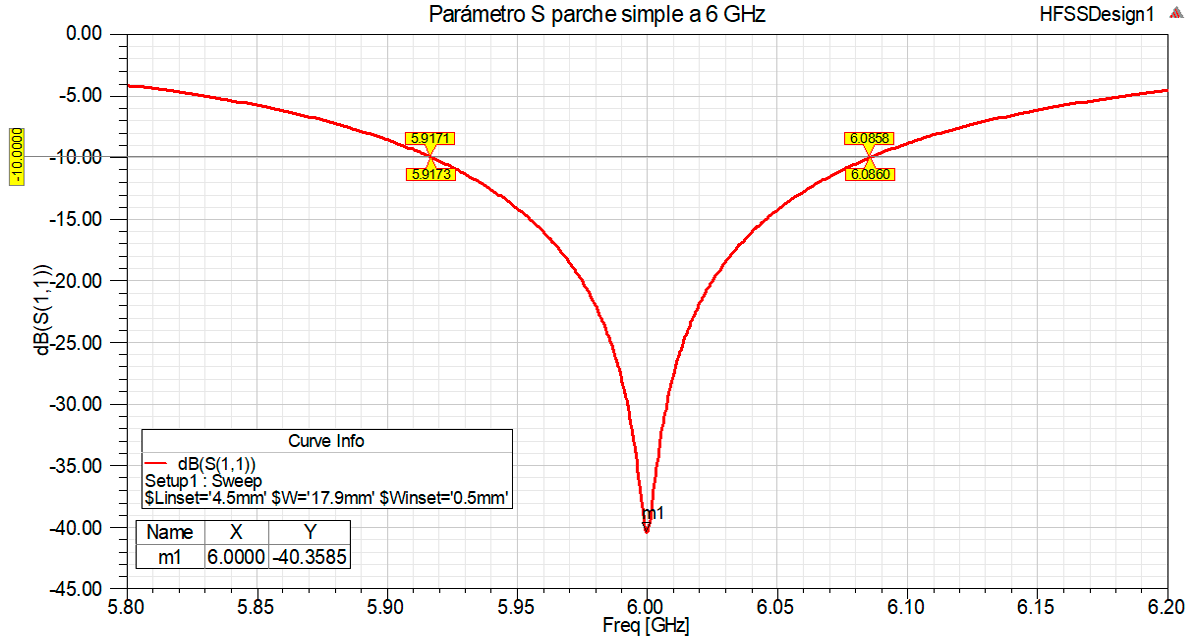
\includegraphics[width=\textwidth]{archivos/analisis/1x12/1}
        \caption{Parámetro $S_{11}$ para el parche simple a 6 GHz}
        \label{fig:s1x12}
\end{figure}

\subsection{Reactancia}
\par La curva de reactancia arroja un valor a la frecuencia de trabajo de -0.63 $\Omega$. Muy cerca del valor esperado, 0.
\\
\begin{figure}[H]
    \centering
        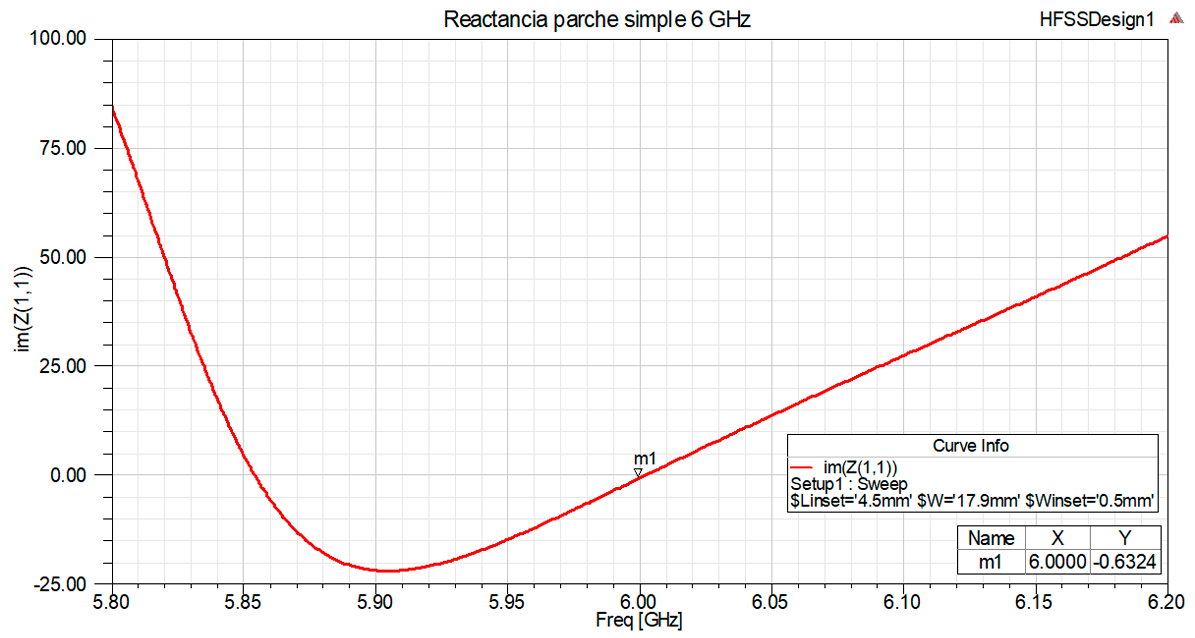
\includegraphics[width=0.85\textwidth]{archivos/analisis/1x12/2}
        \caption{Reactancia para el parche simple a 6 GHz}
        \label{fig:react1x12}
\end{figure}


\subsection{Resistencia}
\par La parte real de la impedancia ofrece un valor a la frecuencia de trabajo de 49.28 $\Omega$. Muy cerca del valor esperado, 50, con un error de tan solo el 1.44\%.
\\
\begin{figure}[H]
    \centering
        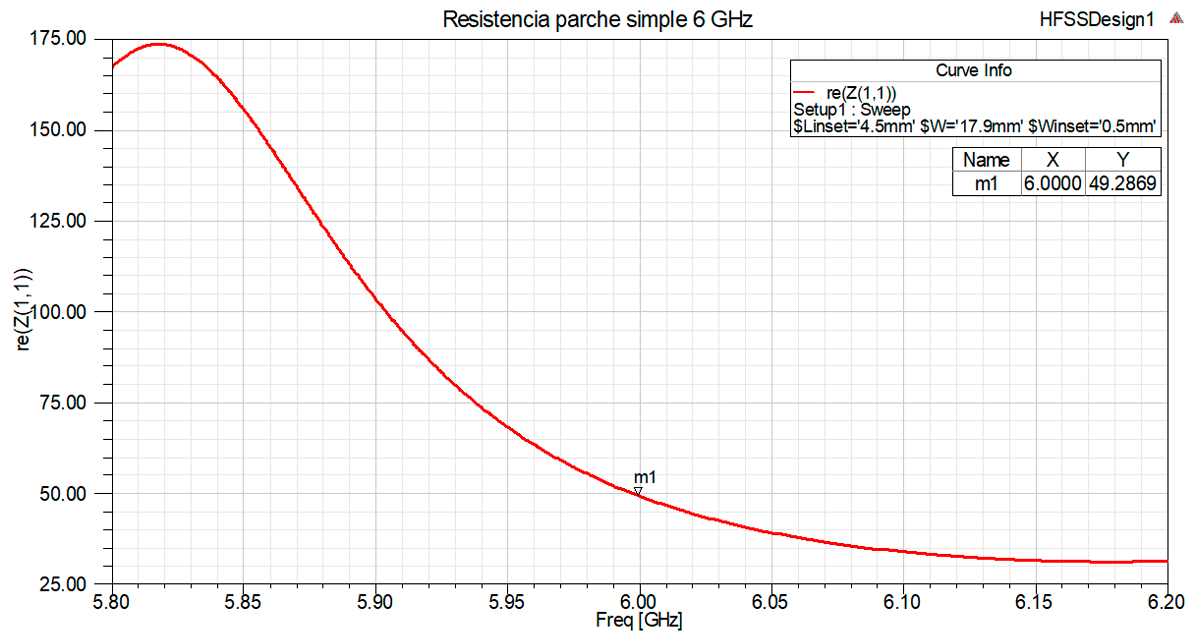
\includegraphics[width=0.85\textwidth]{archivos/analisis/1x12/3}
        \caption{Resistencia para el parche simple a 6 GHz}
        \label{fig:resis1x12}
\end{figure}


\subsection{Patrón de radiación}
\par En cuanto a los patrones de radiación, se puede observar como, al igual que el parche simple a 2.4 GHz, el patrón de radiación es omnidireccional para el plano superior de la antena, y no se ve afectado por ningún otro tipo de elemento radiante. La directividad para el ángulo de máxima radiación encontrada es de 7.66 dB.
\\
\subsubsection{Plano E}
\begin{figure}[H]
    \centering
        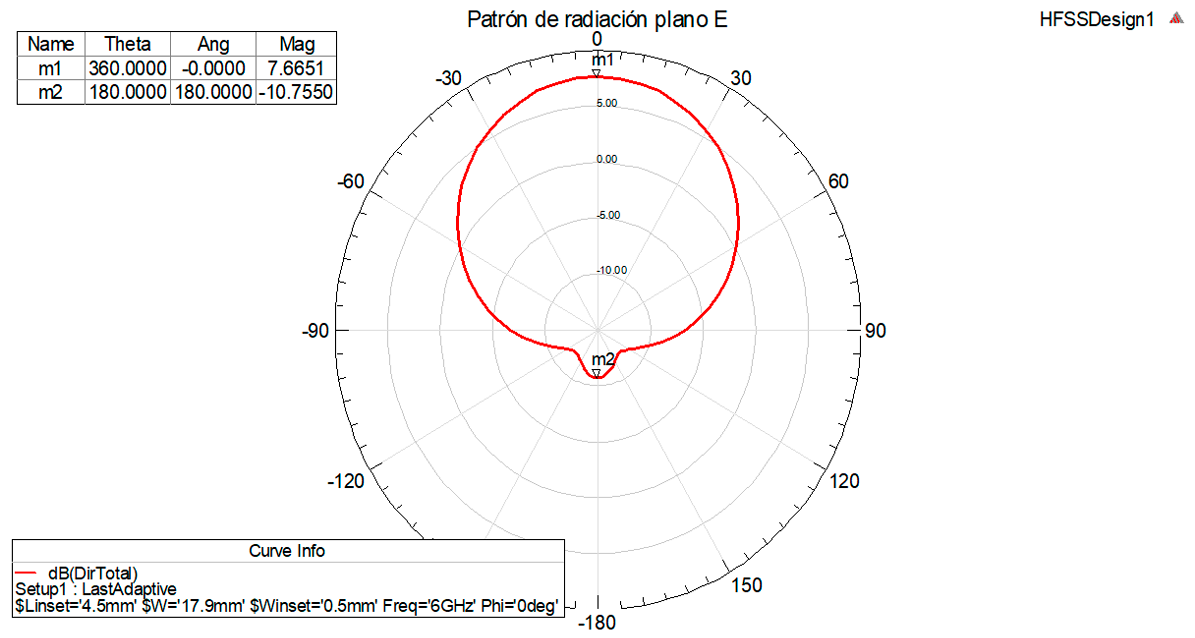
\includegraphics[width=0.8\textwidth]{archivos/analisis/1x12/4}
        \caption{Radiación en el plano E para el parche simple a 6 GHz}
        \label{fig:E1x12}
\end{figure}

\subsubsection{Plano H}
\begin{figure}[H]
    \centering
        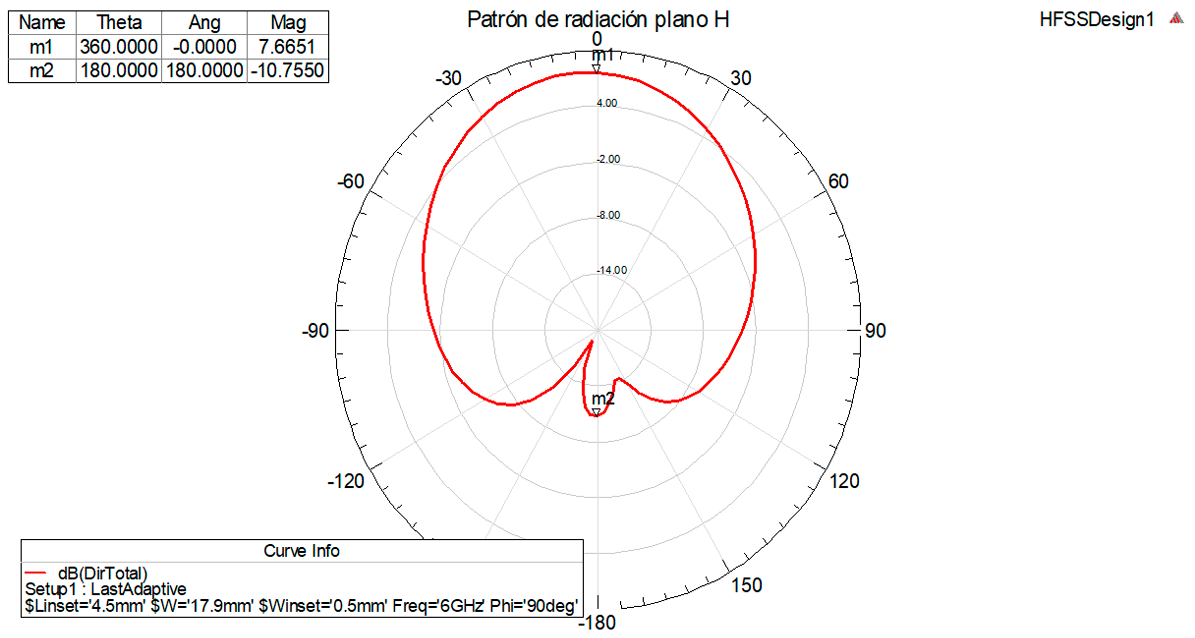
\includegraphics[width=0.8\textwidth]{archivos/analisis/1x12/5}
        \caption{Radiación en el plano H para el parche simple a 6 GHz}
        \label{fig:H1x12}
\end{figure}

\newpage
\subsection{Radiación 3D}
\par Mediante el diagrama de radiación 3D se puede observar el comportamiento omnidireccional de la antena. 

\begin{figure}[H]
     \centering
     \begin{subfigure}[b]{0.75\textwidth}
         \centering
         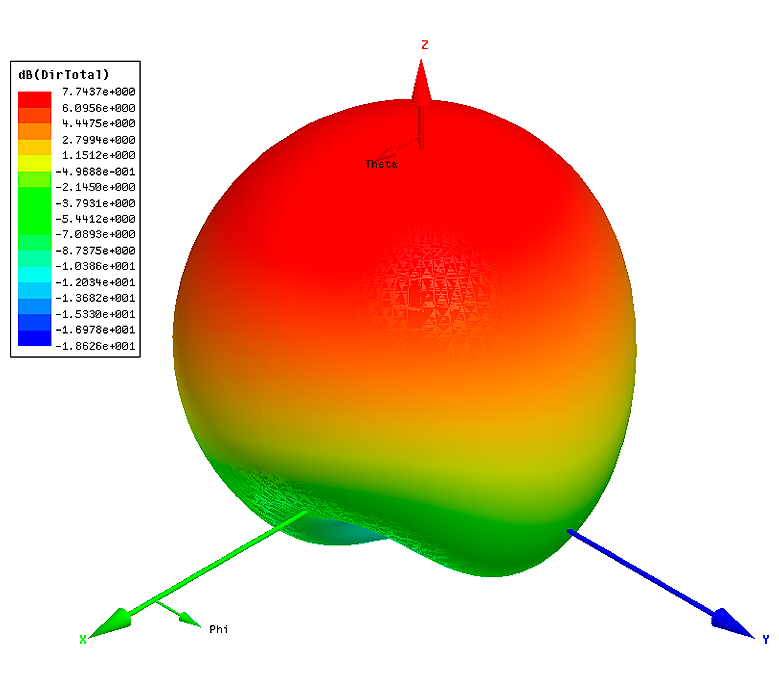
\includegraphics[width=0.85\textwidth]{archivos/analisis/1x12/6}
         \caption{Representación isométrica del diagrama de radiación 3D}
         \label{fig:3d11x12}
     \end{subfigure}
     \hfill
     \begin{subfigure}[b]{0.75\textwidth}
         \centering
         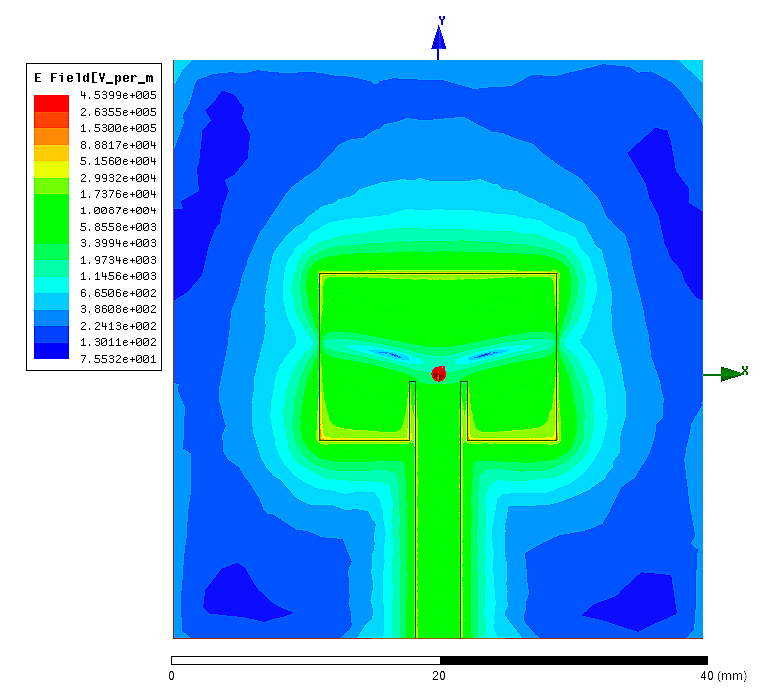
\includegraphics[width=0.85\textwidth]{archivos/analisis/1x12/7}
         \caption{Representación superior del diagrama de radiación 3D}
         \label{fig:3d21x12}
     \end{subfigure}
     \hfill
        \caption{Radiación 3D para el parche simple a 6 GHz}
        \label{fig:3d1x12}
\end{figure}

\newpage
\subsection{Campo eléctrico}
\par Finalmente, podemos observar la distribución de campos eléctricos en el parche. 

\begin{figure}[H]
    \centering
        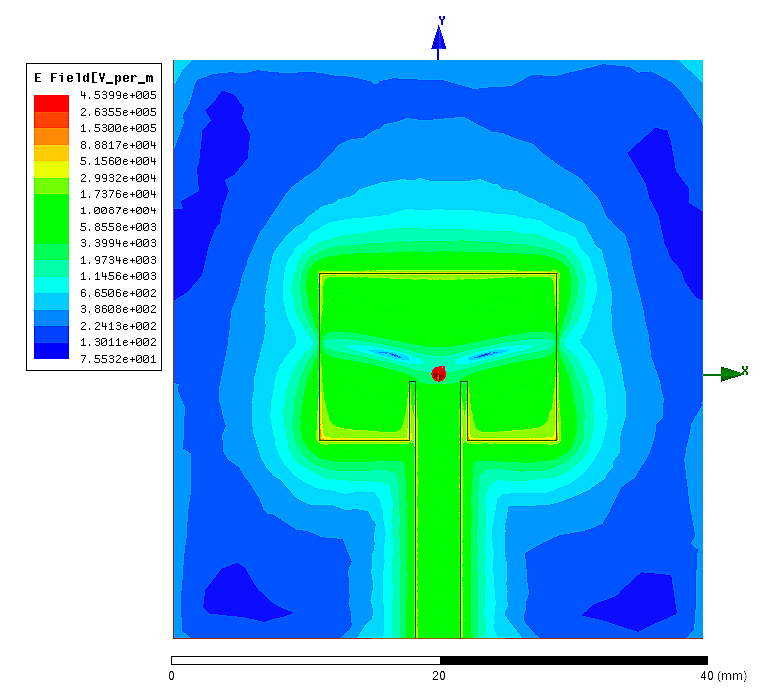
\includegraphics[width=\textwidth]{archivos/analisis/1x12/8}
        \caption{Distribución de campos eléctricos para el parche simple a 6 GHz}
        \label{fig:elec1x12}
\end{figure}


\subsection{Resumen}
\par Como se puede observar en este parche único a 6 GHz, los resultados obtenidos son muy similares a los obtenidos en el caso de 2.4 GHz. El patrón de radiación de la antena se caracteriza por el ser el más básico que podemos encontrar en una antena de tipo microstrip, además de tratarse de un patrón muy útil para aplicaciones móviles puesto que su característica omnidireccional se adapta a los casos de uso en los que el patrón de radiación de la antena no esté apuntando directamente a la antena de telefonía. 
\\
\par En la tabla \ref{tab:res1x12} se pueden observar un resumen de los parámetros característicos de la antena. En ella se puede observar el buen rendimiento obtenido

\begin{table}[H]
  
  
   \small % text size of table content
   \centering % center the table
   \begin{tabular}{c c} % alignment of each column data
   \toprule[\heavyrulewidth]\toprule[\heavyrulewidth]
   \textbf{Parámetro} & \textbf{Parche simple 6 GHz} \\ 
   \midrule
   \textbf{$S_{11}$} & -40.35 dB \\
   \textbf{Ancho de banda} & 168 MHz \\
   \textbf{Directividad} & 7.66 dB \\
   \textbf{Ganancia} & 7.41 dB \\
   \textbf{Eficiencia de radiación} & 93.15\% \\
   \textbf{Relación delante/atrás} & 18.42 dB \\

   \bottomrule[\heavyrulewidth] 
   \end{tabular}
   \caption{Parámetros característicos del parche único microstrip a 6 GHz} 
    \label{tab:res1x12}
\end{table}









\section{Array 2x1 a 2.4 GHz}
\par Para el array en configuración 2x1 a 2.4 GHz los resultados obtenidos son los siguientes:

\subsection{Pérdidas de retorno}
\par En cuanto a su curva de pérdidas de retorno del array a 2.4 GHz, se puede observar un valor pico de -36.46 dB y un ancho de banda de 34.3 MHz, desde los 2.3835 GHz hasta los 2.4173 GHz, lo que equivale a un 1.43\% de la frecuencia de trabajo.
\\
\begin{figure}[H]
    \centering
        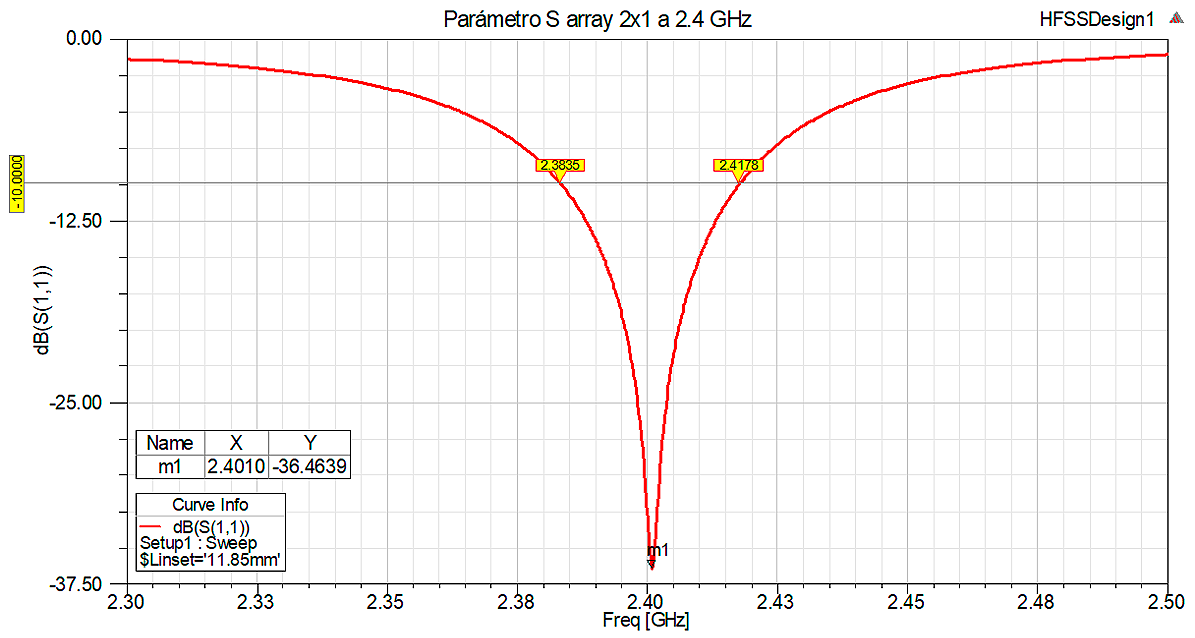
\includegraphics[width=\textwidth]{archivos/analisis/2x11/1}
        \caption{Parámetro $S_{11}$ para el array 2x1 a 2.4 GHz}
        \label{fig:s2x11}
\end{figure}

\subsection{Reactancia}
\par La curva de reactancia arroja un valor a la frecuencia de trabajo de -1.37 $\Omega$. 
\\
\begin{figure}[H]
    \centering
        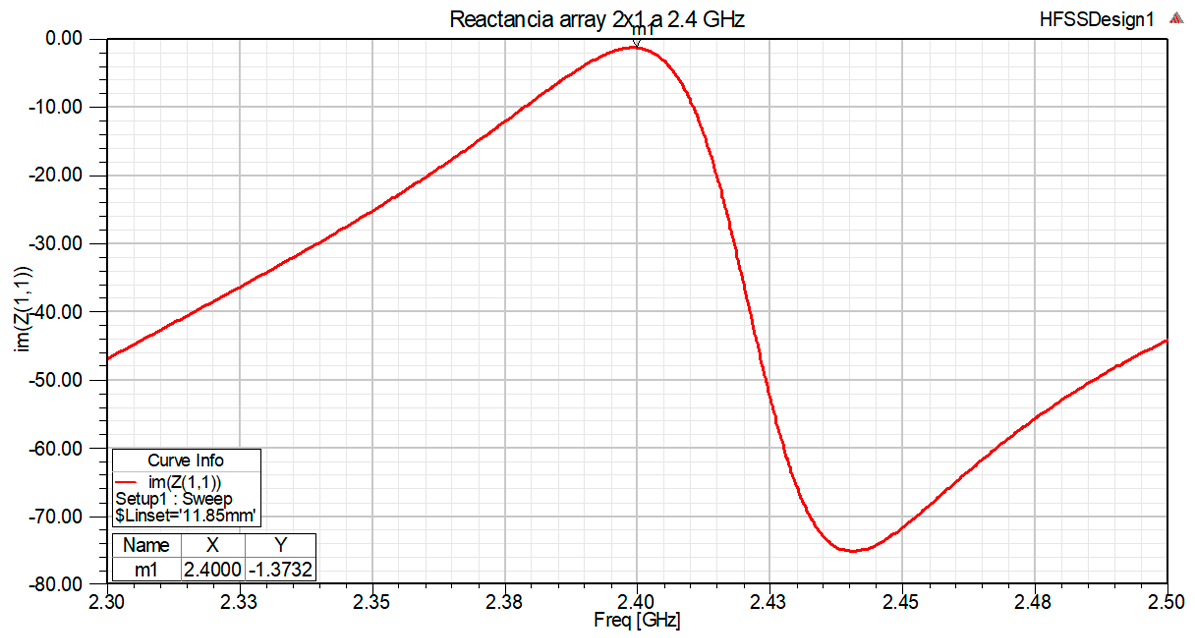
\includegraphics[width=0.85\textwidth]{archivos/analisis/2x11/2}
        \caption{Reactancia para el array 2x1 a 2.4 GHz}
        \label{fig:react2x11}
\end{figure}

\subsection{Resistencia}
\par La parte real de la impedancia ofrece un valor a la frecuencia de trabajo de 48.12 $\Omega$.
\\
\begin{figure}[H]
    \centering
        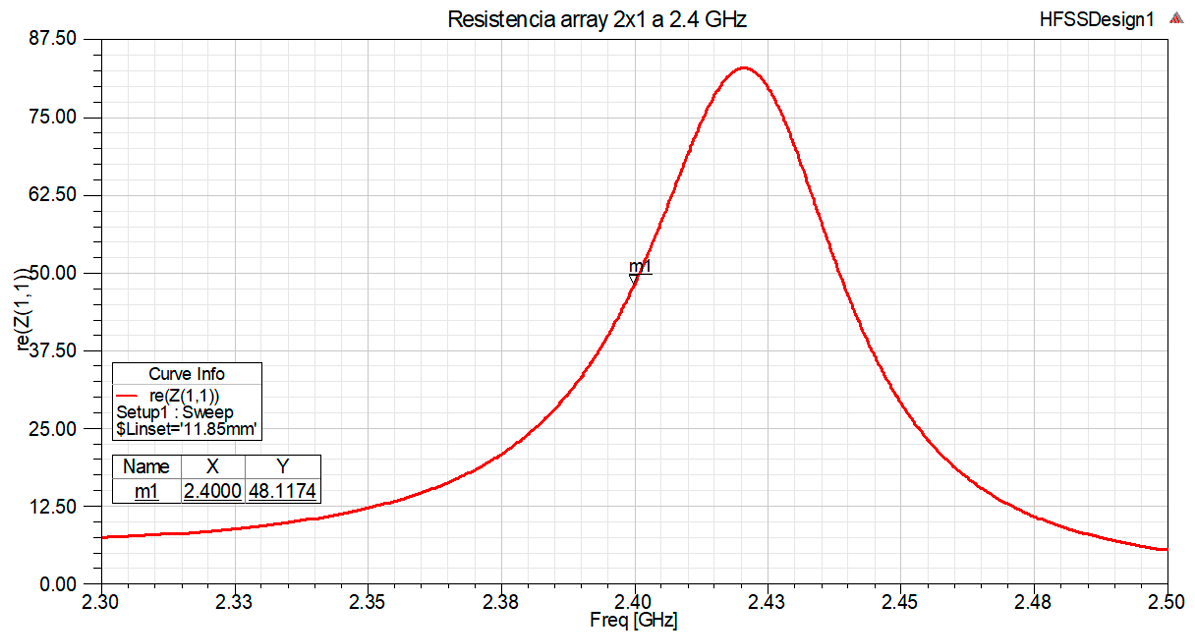
\includegraphics[width=0.85\textwidth]{archivos/analisis/2x11/3}
        \caption{Resistencia para el array 2x1 a 2.4 GHz}
        \label{fig:resis2x11}
\end{figure}

\subsection{Patrón de radiación}
\par En cuanto a los patrones de radiación, se puede observar se puede observar un comportamiento más directivo con unos lóbulos laterales y trasero de bastante magnitud en relación al lóbulo principal para el plano E, mientras que en el plano H se observa un comportamiento completamente omnidireccional para el plano superior del array. La directividad en el ángulo de máxima radiación observada es de 7.64 dB.
\\
\subsubsection{Plano E}
\begin{figure}[H]
    \centering
        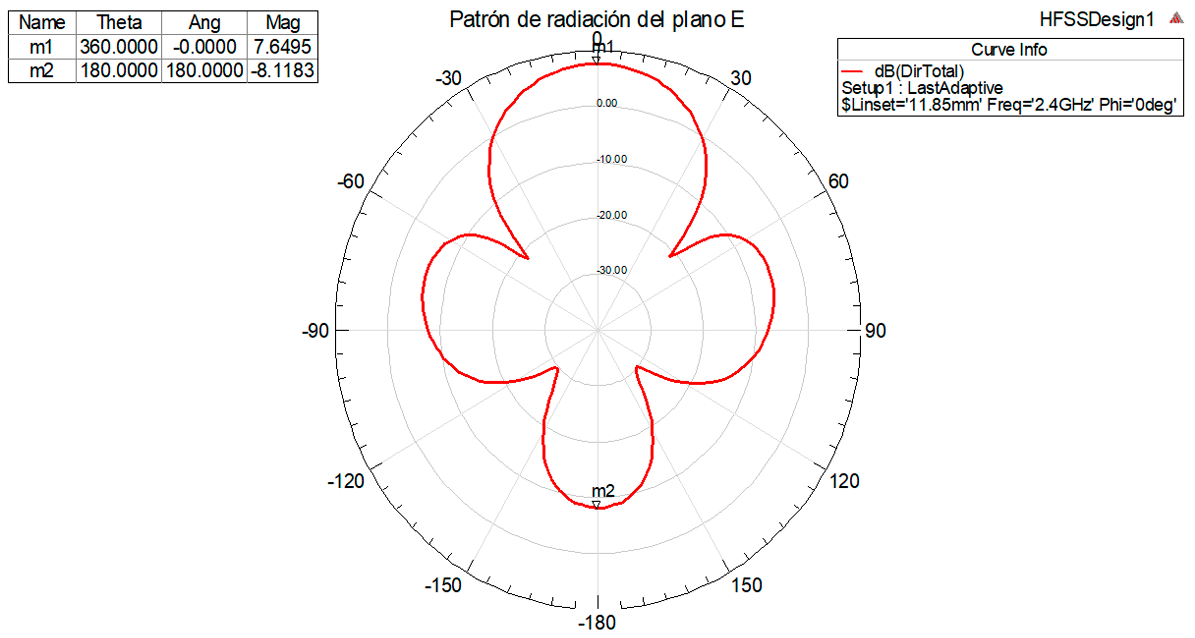
\includegraphics[width=0.75\textwidth]{archivos/analisis/2x11/4}
        \caption{Radiación en el plano E para el array 2x1 a 2.4 GHz}
        \label{fig:E2x11}
\end{figure}

\subsubsection{Plano H}
\begin{figure}[H]
    \centering
        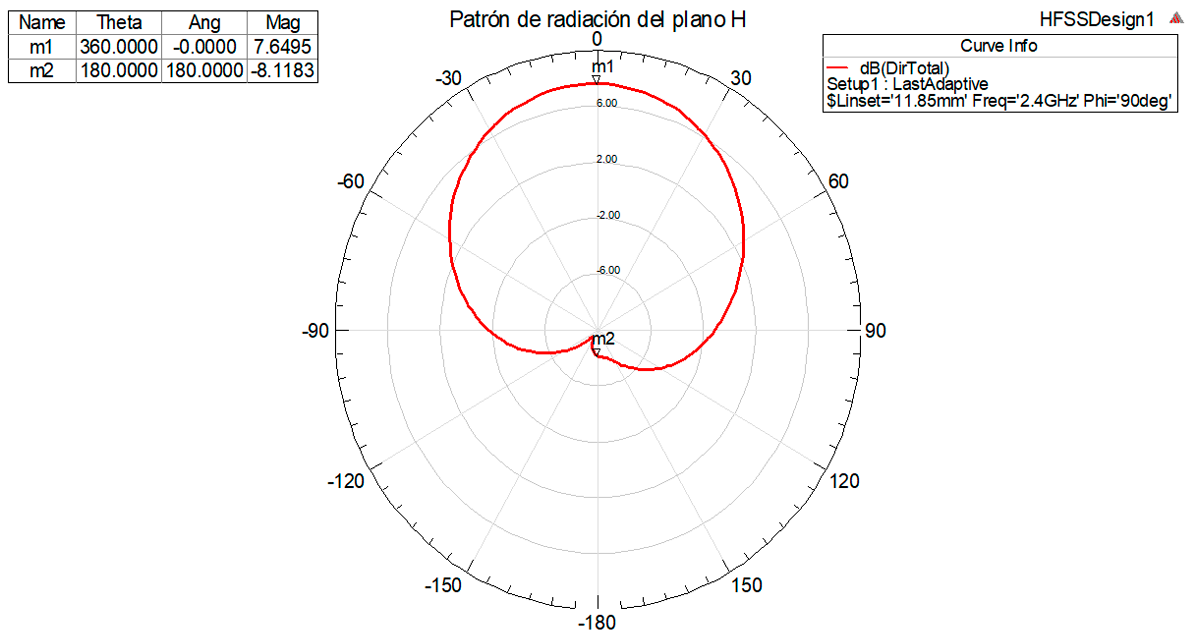
\includegraphics[width=0.75\textwidth]{archivos/analisis/2x11/5}
        \caption{Radiación en el plano H para el array 2x1 a 2.4 GHz}
        \label{fig:H2x11}
\end{figure}

\subsection{Radiación 3D}
\par Mediante el diagrama de radiación 3D se puede observar el comportamiento directivo en el plano perpendicular a la configuración del array, producido por la superposición de la radiación de ambos parches.

\begin{figure}[H]
     \centering
     \begin{subfigure}[b]{0.7\textwidth}
         \centering
         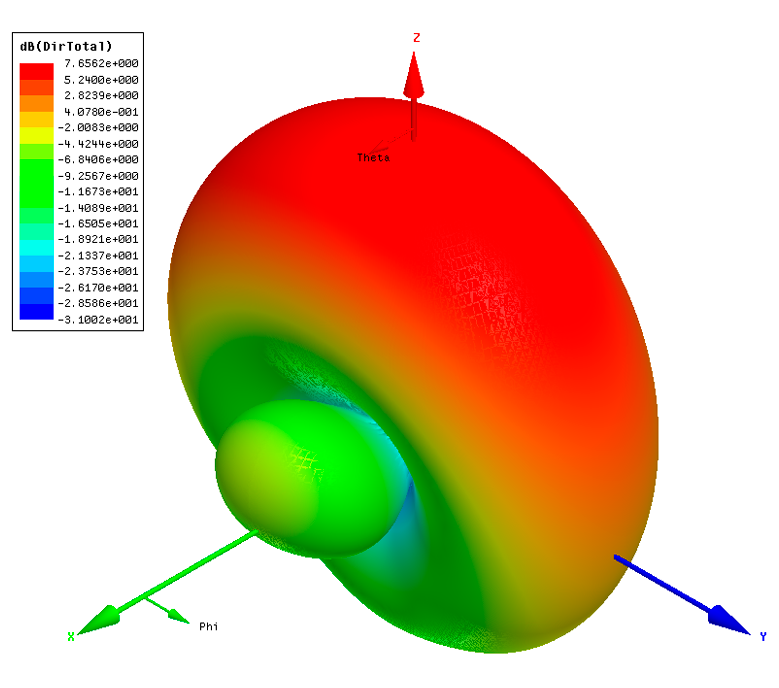
\includegraphics[width=0.85\textwidth]{archivos/analisis/2x11/6}
         \caption{Representación isométrica del diagrama de radiación 3D}
         \label{fig:3d12x11}
     \end{subfigure}
     \hfill
     \begin{subfigure}[b]{0.7\textwidth}
         \centering
         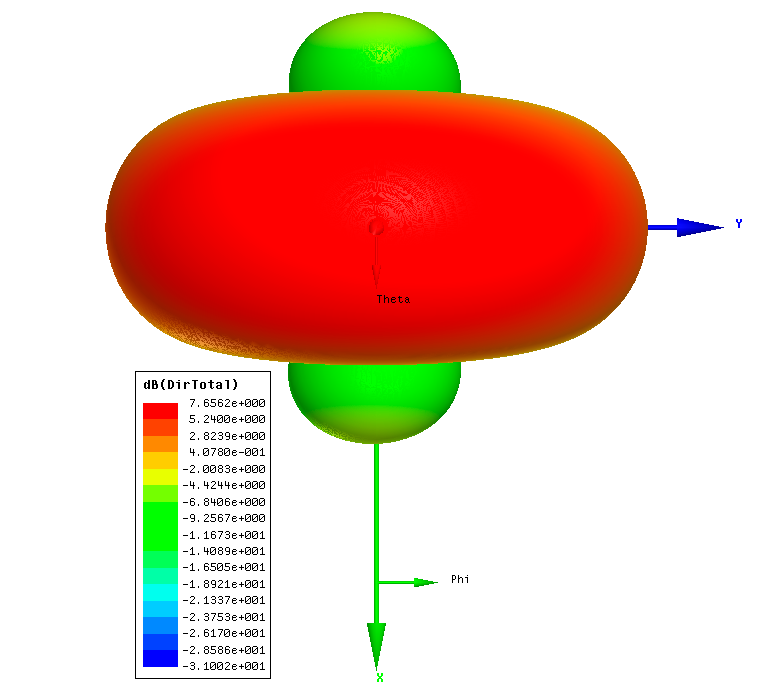
\includegraphics[width=0.85\textwidth]{archivos/analisis/2x11/7}
         \caption{Representación superior del diagrama de radiación 3D}
         \label{fig:3d22x11}
     \end{subfigure}
     \hfill
        \caption{Radiación 3D para el array 2x1 a 2.4 GHz}
        \label{fig:3d2x11}
\end{figure}

\subsection{Campo eléctrico}
\par Finalmente, podemos observar la distribución de campos eléctricos en el parche. 

\begin{figure}[H]
    \centering
        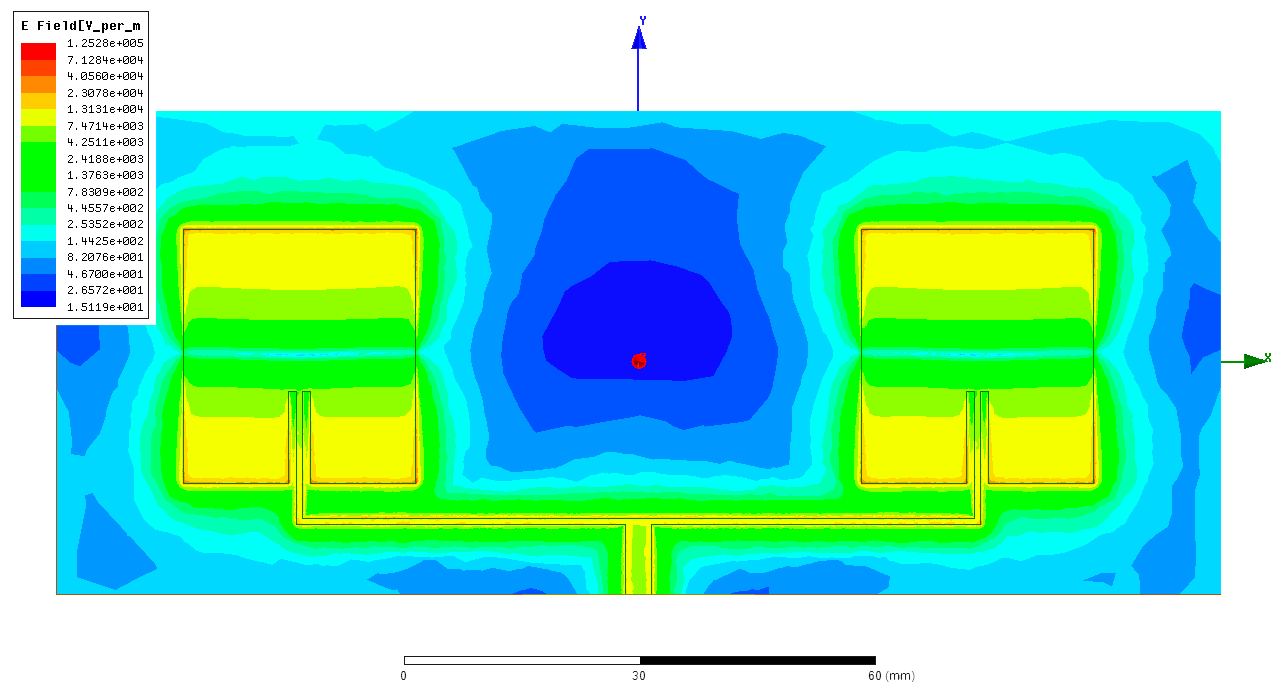
\includegraphics[width=\textwidth]{archivos/analisis/2x11/8}
        \caption{Distribución de campos eléctricos para el para el array 2x1 a 2.4 GHz}
        \label{fig:elec2x11}
\end{figure}

\subsection{Resumen}
\par En esta primera configuración de array a 2.4 GHz se puede observar los primeros comportamientos directivos producidos por la conjunción de diferentes parches en fase funcionando en la misma antena. 
\\
\par En la tabla \ref{tab:res2x11} se pueden observar un resumen de los parámetros característicos de la antena. Como se puede observar, el rendimiento obtenido para esta antena es un tanto menor al obtenido previamente en las\todo{mriar comentario de stephan} antenas de parche único y esto es principalmente debido a la complejidad del proceso de adaptación al aumentar el número de parches en las configuraciones de array.

\begin{table}[H]
  
   
   \small % text size of table content
   \centering % center the table
   \begin{tabular}{c c} % alignment of each column data
   \toprule[\heavyrulewidth]\toprule[\heavyrulewidth]
   \textbf{Parámetro} & \textbf{Array 2x1 a 2.4 GHz} \\ 
   \midrule
   \textbf{$S_{11}$} & -36.46 dB \\
   \textbf{Ancho de banda} & 34.3 MHz \\
   \textbf{Directividad} & 7.64 dB \\
   \textbf{Ganancia} & 7.03 dB \\
   \textbf{Eficiencia de radiación} & 86.94\% \\
   \textbf{Relación delante/atrás} & 15.89 dB \\

   \bottomrule[\heavyrulewidth] 
   \end{tabular}
  
   \caption{Parámetros característicos para el array 2x1 a 2.4 GHz} 
    \label{tab:res2x11}
\end{table}













\section{Array 2x1 a 6 GHz}
\par Para el array en configuración 2x1 a 6 GHz los resultados obtenidos son los siguientes:

\subsection{Pérdidas de retorno}
\par En cuanto a su curva de pérdidas de retorno del array a 6 GHz, se puede observar un valor pico de -76.78 dB y un ancho de banda de 179.1 MHz, desde los 5.9014 GHz hasta los 6.0805 GHz, lo que equivale a un 2.98\% de la frecuencia de trabajo.
\\
\begin{figure}[H]
    \centering
        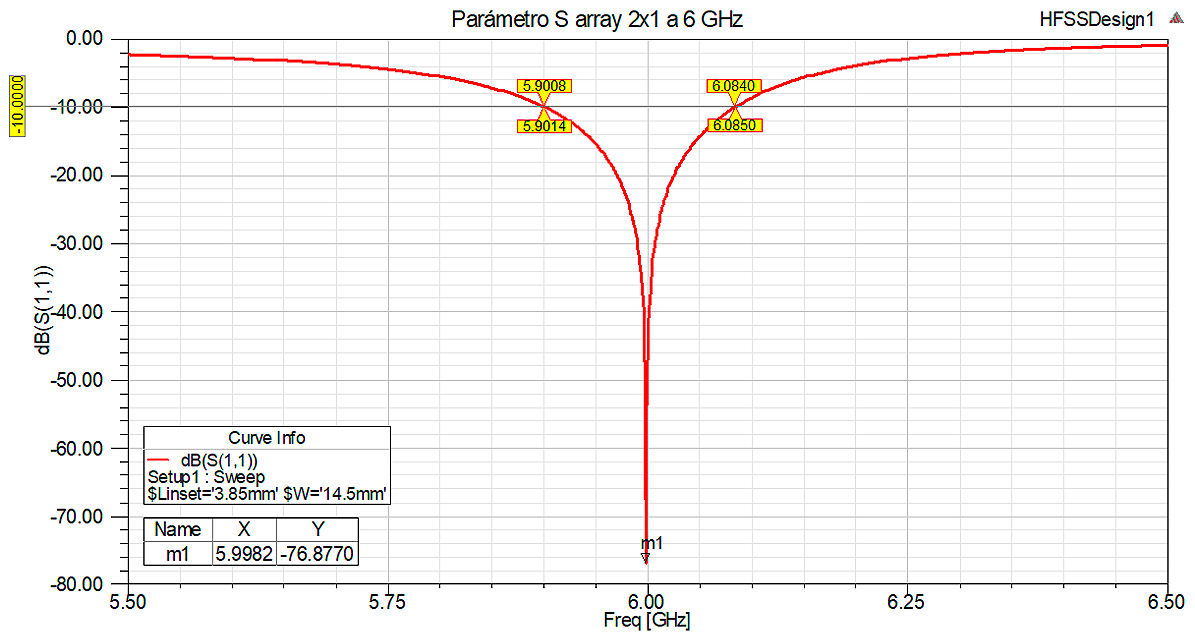
\includegraphics[width=\textwidth]{archivos/analisis/2x12/1}
        \caption{Parámetro $S_{11}$ para el array 2x1 a 6 GHz}
        \label{fig:s2x12}
\end{figure}

\newpage
\subsection{Reactancia}
\par La curva de reactancia arroja un valor a la frecuencia de trabajo de -0.03 $\Omega$. 
\\
\begin{figure}[H]
    \centering
        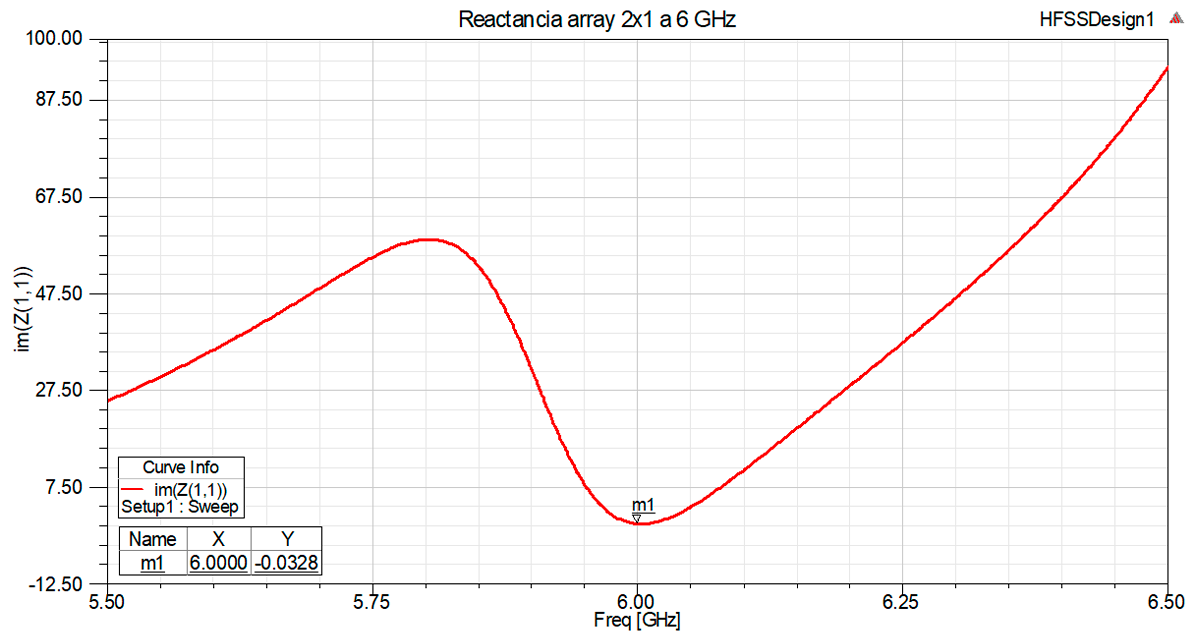
\includegraphics[width=0.85\textwidth]{archivos/analisis/2x12/2}
        \caption{Reactancia para el array 2x1 a 6 GHz}
        \label{fig:react2x12}
\end{figure}

\subsection{Resistencia}
\par La parte real de la impedancia ofrece un valor a la frecuencia de trabajo de 49.35 $\Omega$.
\\
\begin{figure}[H]
    \centering
        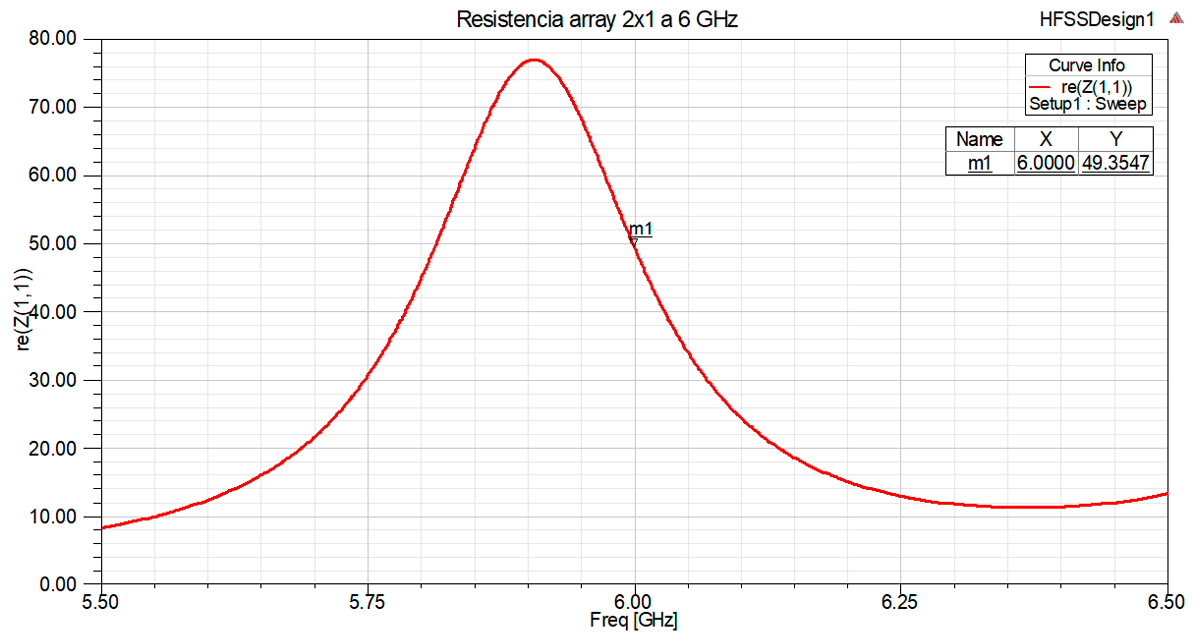
\includegraphics[width=0.85\textwidth]{archivos/analisis/2x12/3}
        \caption{Resistencia para el array 2x1 a 6 GHz}
        \label{fig:resis2x12}
\end{figure}

\subsection{Patrón de radiación}
\par En este caso se puede observar el mismo patrón de radiación base que se encontró en el array 2x1 a 6 GHz pero con una directividad aumentada del lóbulo principal con respecto a los lóbulos secundarios y traseros, con un pico de directividad en el ángulo de máxima radiación de 9.97 dB. 
\\
\subsubsection{Plano E}
\begin{figure}[H]
    \centering
        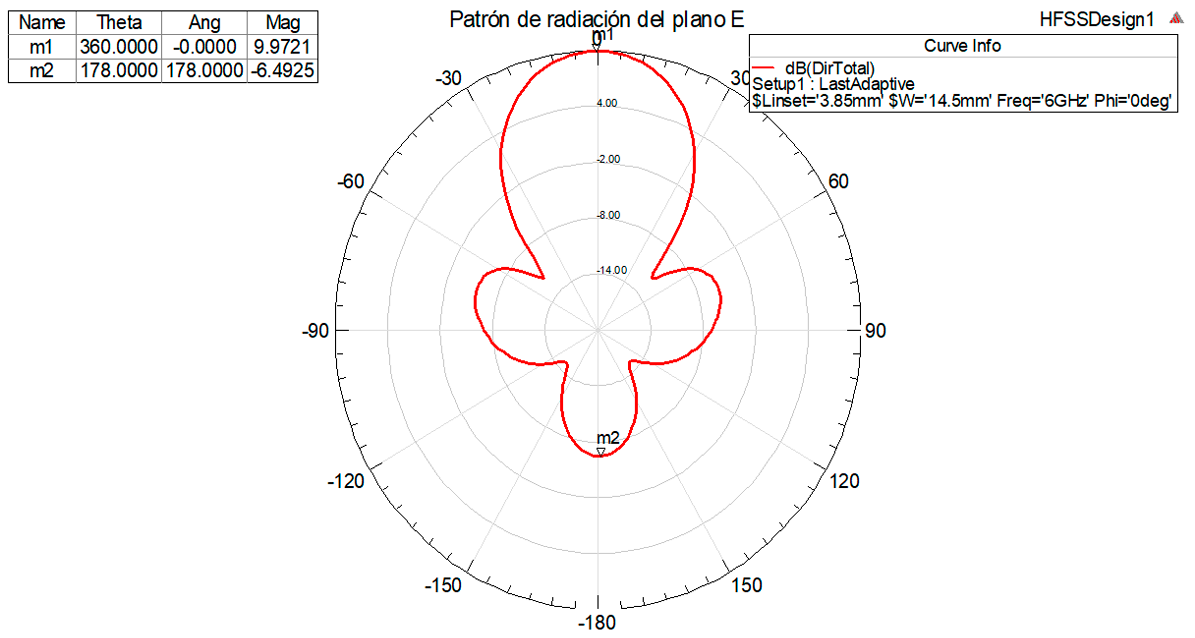
\includegraphics[width=0.8\textwidth]{archivos/analisis/2x12/4}
        \caption{Radiación en el plano E para el array 2x1 a 6 GHz}
        \label{fig:E2x12}
\end{figure}

\subsubsection{Plano H}
\begin{figure}[H]
    \centering
        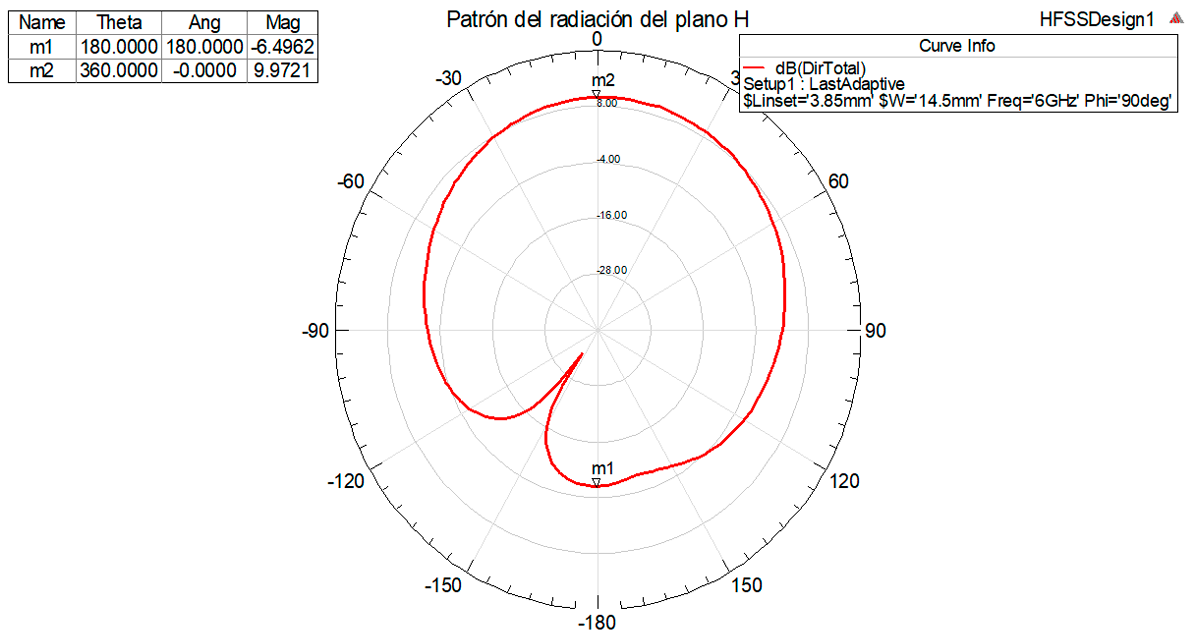
\includegraphics[width=0.8\textwidth]{archivos/analisis/2x12/5}
        \caption{Radiación en el plano H para el array 2x1 a 6 GHz}
        \label{fig:H2x12}
\end{figure}

\subsection{Radiación 3D}
\par Mediante el diagrama de radiación 3D se puede observar, de nuevo, el mismo comportamiento directivo que encontramos en el array a 2.4 GHz de la misma configuración, pero con ese aumento de directividad sobre el lóbulo principal, dejando a los lóbulos laterales en un segundo plano en cuanto a la radiación que estos ofrecen.

\begin{figure}[H]
     \centering
     \begin{subfigure}[b]{0.7\textwidth}
         \centering
         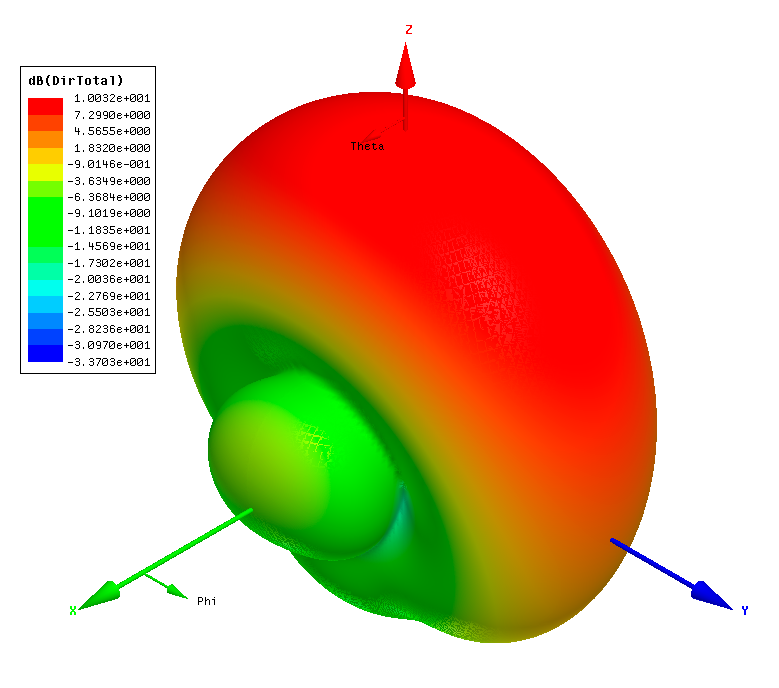
\includegraphics[width=0.85\textwidth]{archivos/analisis/2x12/6}
         \caption{Representación isométrica del diagrama de radiación 3D}
         \label{fig:3d12x12}
     \end{subfigure}
     \hfill
     \begin{subfigure}[b]{0.7\textwidth}
         \centering
         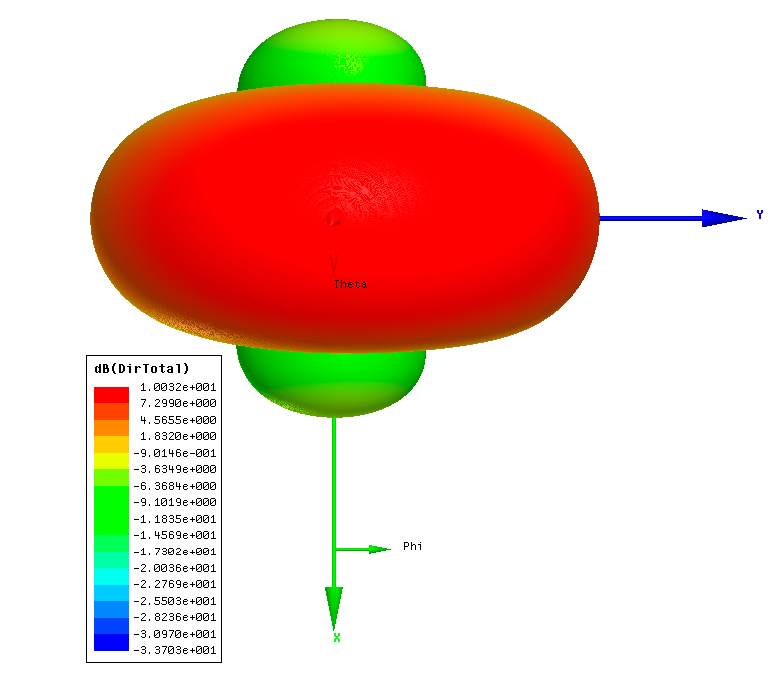
\includegraphics[width=0.85\textwidth]{archivos/analisis/2x12/7}
         \caption{Representación superior del diagrama de radiación 3D}
         \label{fig:3d22x12}
     \end{subfigure}
     \hfill
        \caption{Radiación 3D para el array 2x1 a 6 GHz}
        \label{fig:3d2x12}
\end{figure}

\subsection{Campo eléctrico}
\par Finalmente, podemos observar la distribución de campos eléctricos en el parche. 

\begin{figure}[H]
    \centering
        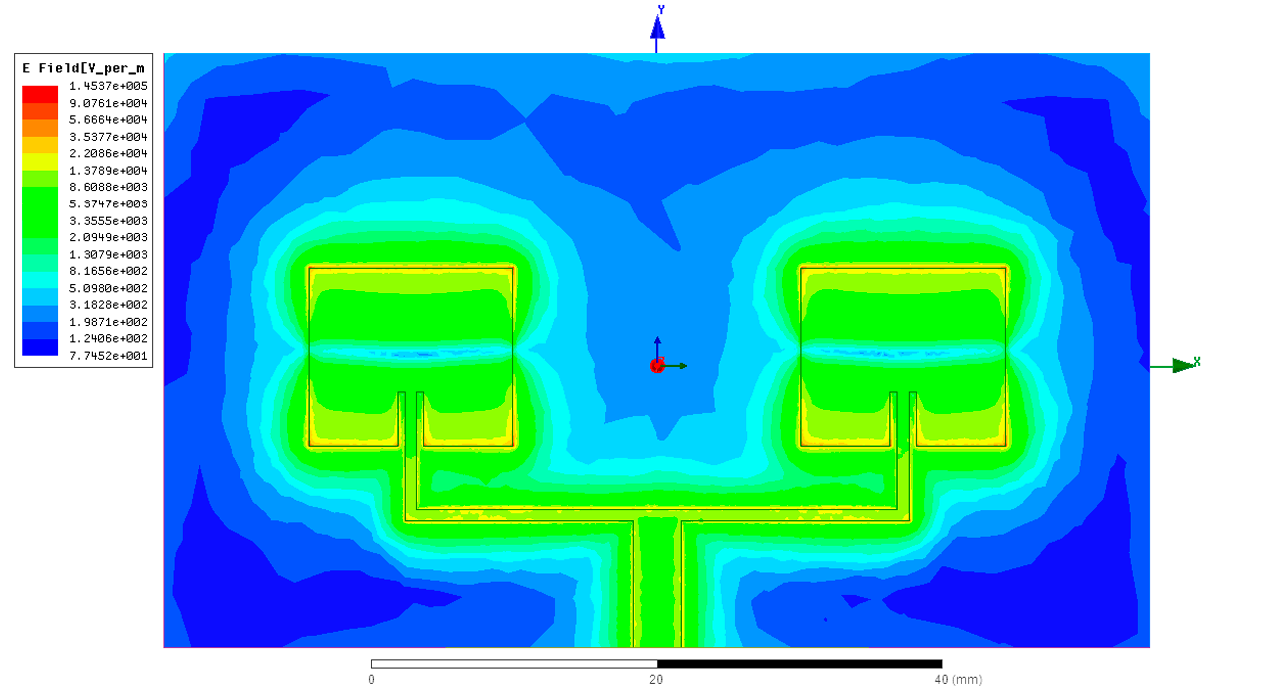
\includegraphics[width=\textwidth]{archivos/analisis/2x12/8}
        \caption{Distribución de campos eléctricos para el para el array 2x1 a 6 GHz}
        \label{fig:elec2x12}
\end{figure}

\subsection{Resumen}
\par En la configuración 2x1 a 6 GHz se puede observar una mejora de parámetros característicos de la antena con respecto a los obtenidos para la antena de 2.4 GHz en la misma configuración. Esto es principalmente debido a la mejor adaptación que ha tenido esta antena entre el conjunto de líneas microstrip que la alimentan.
\\
\par En la tabla \ref{tab:res2x12} se pueden observar un resumen de los parámetros característicos de la antena.

\begin{table}[H]
  
   
   \small % text size of table content
   \centering % center the table
   \begin{tabular}{c c} % alignment of each column data
   \toprule[\heavyrulewidth]\toprule[\heavyrulewidth]
   \textbf{Parámetro} & \textbf{Array 2x1 a 6 GHz} \\ 
   \midrule
   \textbf{$S_{11}$} & -76.87 dB \\
   \textbf{Ancho de banda} & 179.1 MHz \\
   \textbf{Directividad} & 9.97 dB \\
   \textbf{Ganancia} & 9.77 dB \\
   \textbf{Eficiencia de radiación} & 94.14\% \\
   \textbf{Relación delante/atrás} & 16.64 dB \\

   \bottomrule[\heavyrulewidth] 
   \end{tabular}
   
   \caption{Parámetros característicos del array 2x1 a 6 GHz} 
   \label{tab:res2x12}
\end{table}


















\section{Array 2x2 a 2.4 GHz}
\par Para el array en configuración 2x2 a 2.4 GHz los resultados obtenidos son los siguientes:

\subsection{Pérdidas de retorno}
\par En cuanto a su curva de pérdidas de retorno del array a 2.4 GHz, se puede observar un valor pico de -40.70 dB y un ancho de banda de 34.6 MHz, desde los 2.4161 GHz hasta los 2.3815 GHz, lo que equivale a un 1.44\% de la frecuencia de trabajo.
\\
\begin{figure}[H]
    \centering
        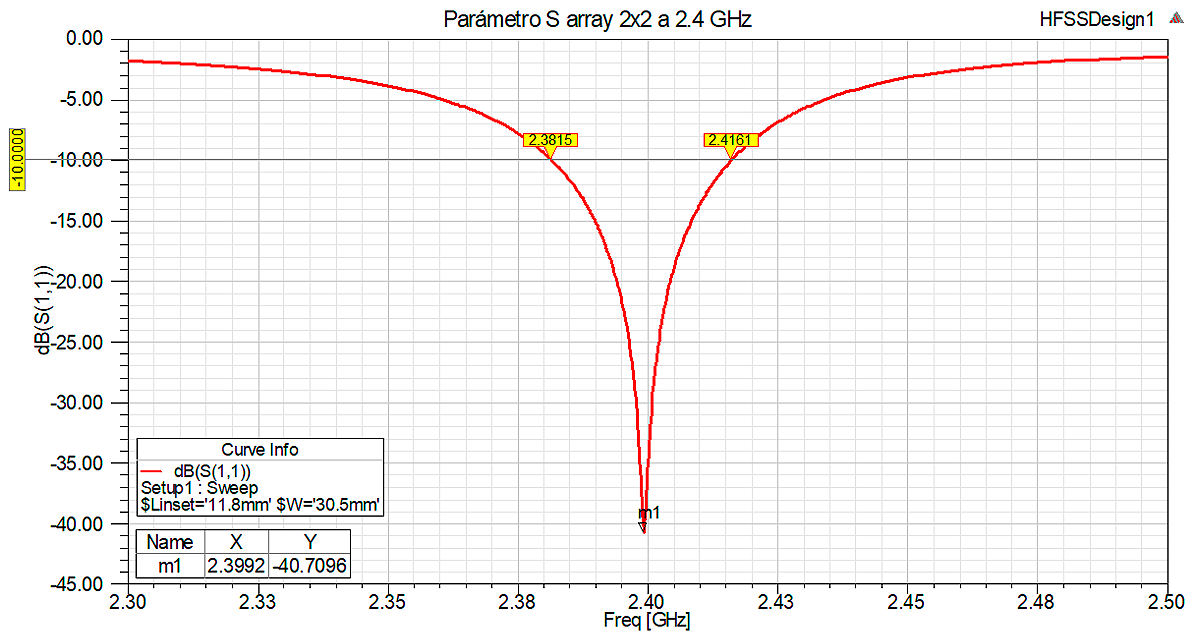
\includegraphics[width=\textwidth]{archivos/analisis/2x21/1}
        \caption{Parámetro $S_{11}$ para el array 2x2 a 2.4 GHz}
        \label{fig:s2x21}
\end{figure}

\newpage
\subsection{Reactancia}
\par La curva de reactancia arroja un valor a la frecuencia de trabajo de -0.32 $\Omega$. 
\\
\begin{figure}[H]
    \centering
        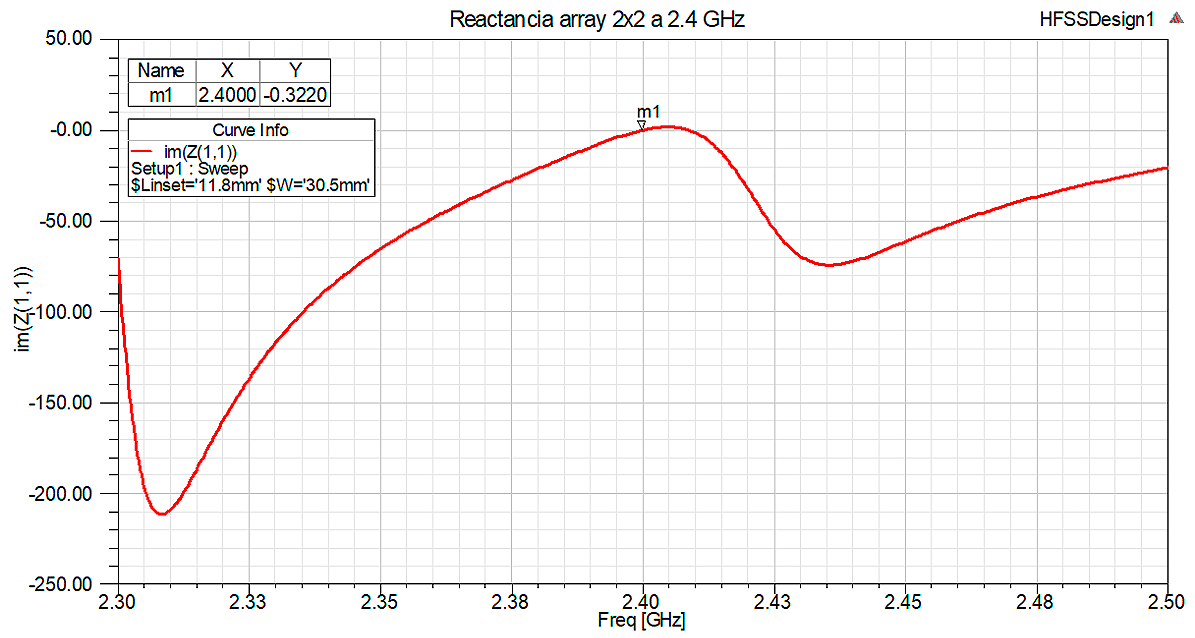
\includegraphics[width=0.8\textwidth]{archivos/analisis/2x21/2}
        \caption{Reactancia para el array 2x2 a 2.4 GHz}
        \label{fig:react2x21}
\end{figure}

\subsection{Resistencia}
\par La parte real de la impedancia ofrece un valor a la frecuencia de trabajo de 51.78 $\Omega$.
\\
\begin{figure}[H]
    \centering
        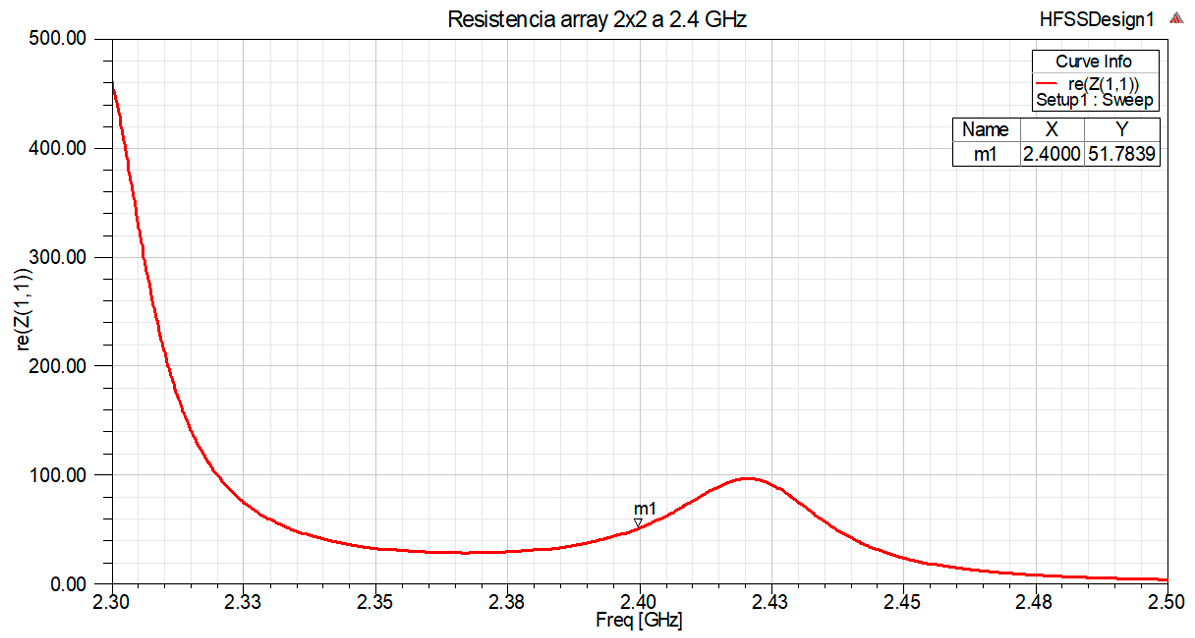
\includegraphics[width=0.8\textwidth]{archivos/analisis/2x21/3}
        \caption{Resistencia para el array 2x2 a 2.4 GHz}
        \label{fig:resis2x21}
\end{figure}

\subsection{Patrón de radiación}
\par El patrón de radiación que se observa es completamente simétrico en el plano E, donde se encuentra un lóbulo principal poco con un máximo de 10.74 dB de directividad. Existen también dos lóbulos laterales de menor intensidad. En cuanto al plano H se puede observar un patrón de directividad más omnidireccional ya que los lóbulos laterales y traseros están más integrados en el patrón y no se presencian tantas zonas de radiación nula como en el plano E. 
\\
\subsubsection{Plano E}
\begin{figure}[H]
    \centering
        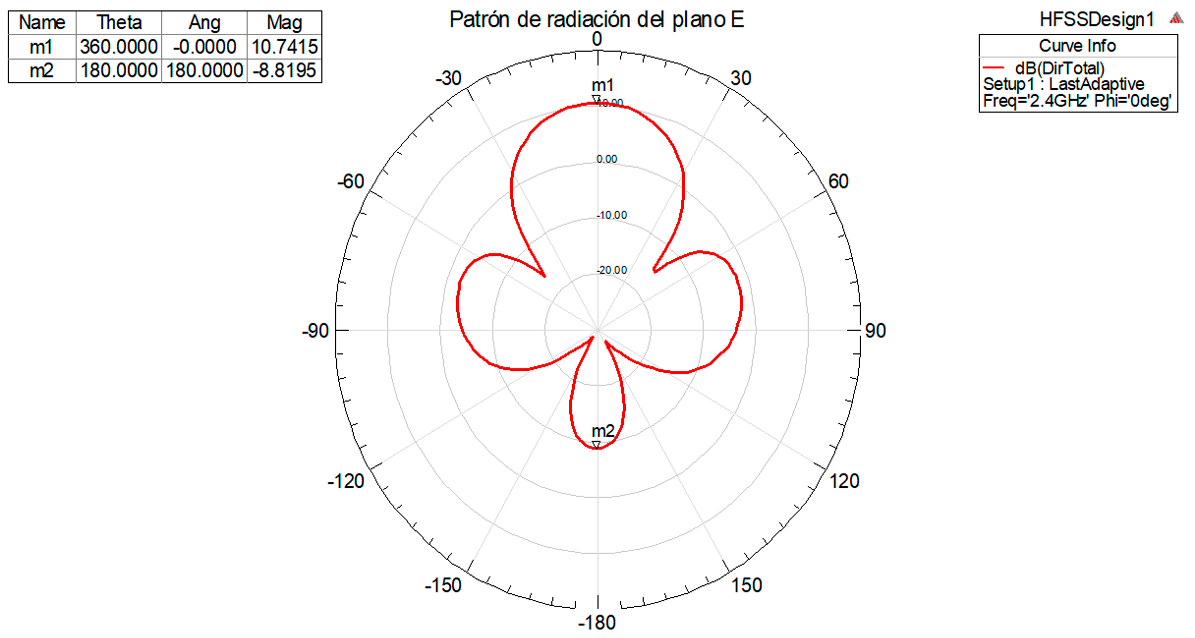
\includegraphics[width=0.75\textwidth]{archivos/analisis/2x21/4}
        \caption{Radiación en el plano E para el array 2x2 a 2.4 GHz}
        \label{fig:E2x21}
\end{figure}

\subsubsection{Plano H}
\begin{figure}[H]
    \centering
        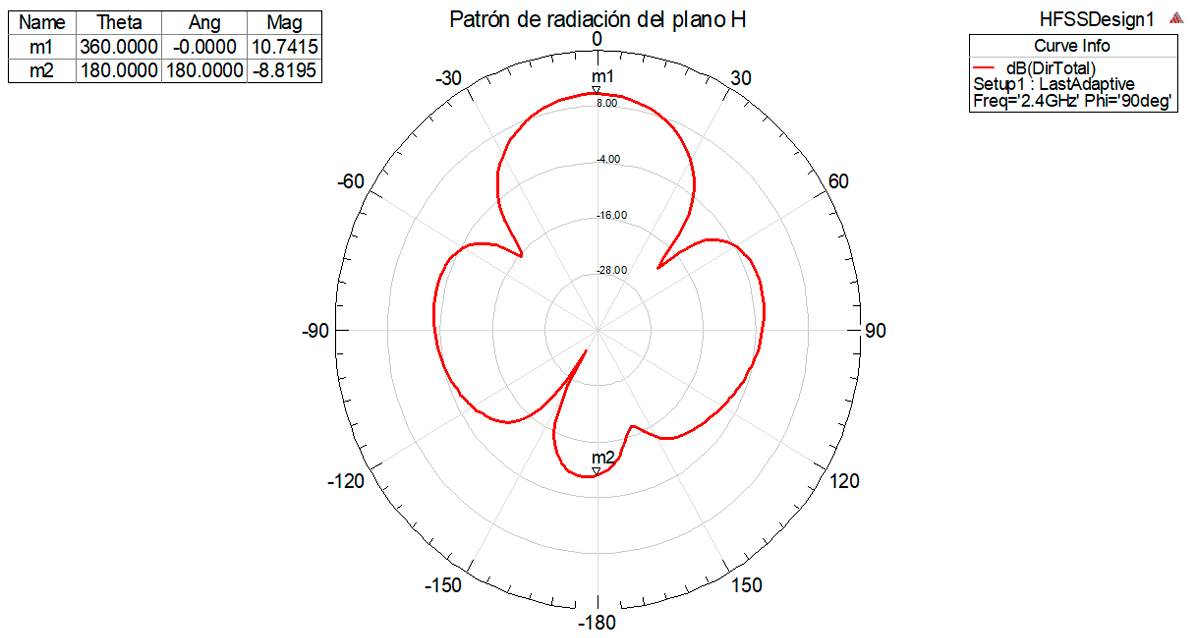
\includegraphics[width=0.75\textwidth]{archivos/analisis/2x21/5}
        \caption{Radiación en el plano H para el array 2x2 a 2.4 GHz}
        \label{fig:H2x21}
\end{figure}

\subsection{Radiación 3D}
\par Desde el diagrama de radiación 3D se puede observar un comportamiento más simétrico del patrón de radiación en su conjunto, donde el cuerpo más presente es el lóbulo principal del patrón y un total de cuatro lóbulos laterales cada 90º alrededor de este.

\begin{figure}[H]
     \centering
     \begin{subfigure}[b]{0.7\textwidth}
         \centering
         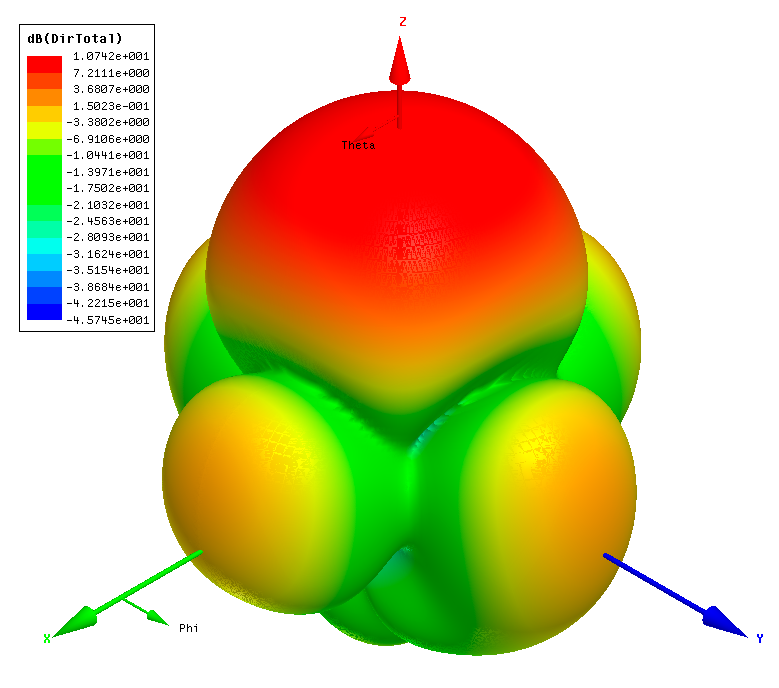
\includegraphics[width=0.85\textwidth]{archivos/analisis/2x21/6}
         \caption{Representación isométrica del diagrama de radiación 3D}
         \label{fig:3d12x21}
     \end{subfigure}
     \hfill
     \begin{subfigure}[b]{0.7\textwidth}
         \centering
         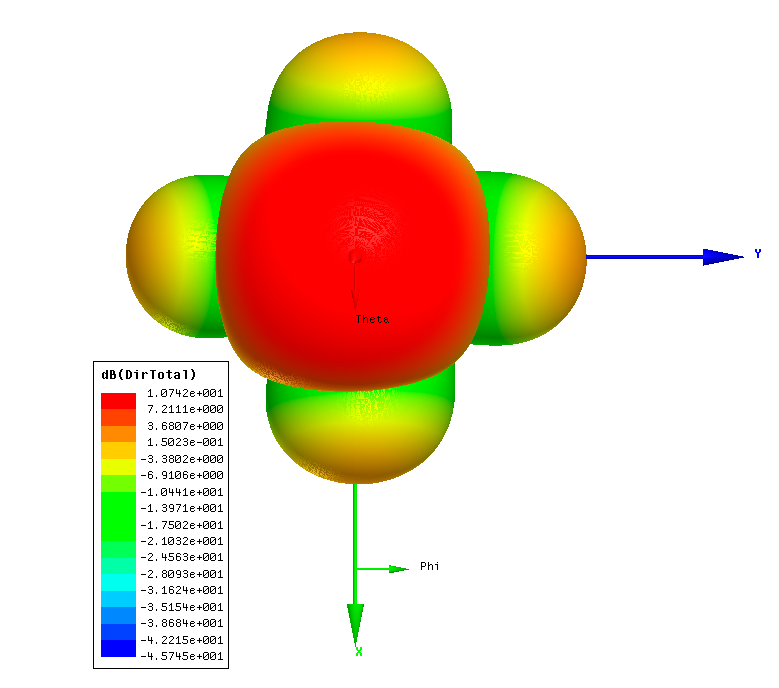
\includegraphics[width=0.85\textwidth]{archivos/analisis/2x21/7}
         \caption{Representación superior del diagrama de radiación 3D}
         \label{fig:3d22x21}
     \end{subfigure}
     \hfill
        \caption{Radiación 3D para el array 2x2 a 2.4 GHz}
        \label{fig:3d2x21}
\end{figure}

\subsection{Campo eléctrico}
\par Finalmente, podemos observar la distribución de campos eléctricos en el parche. 

\begin{figure}[H]
    \centering
        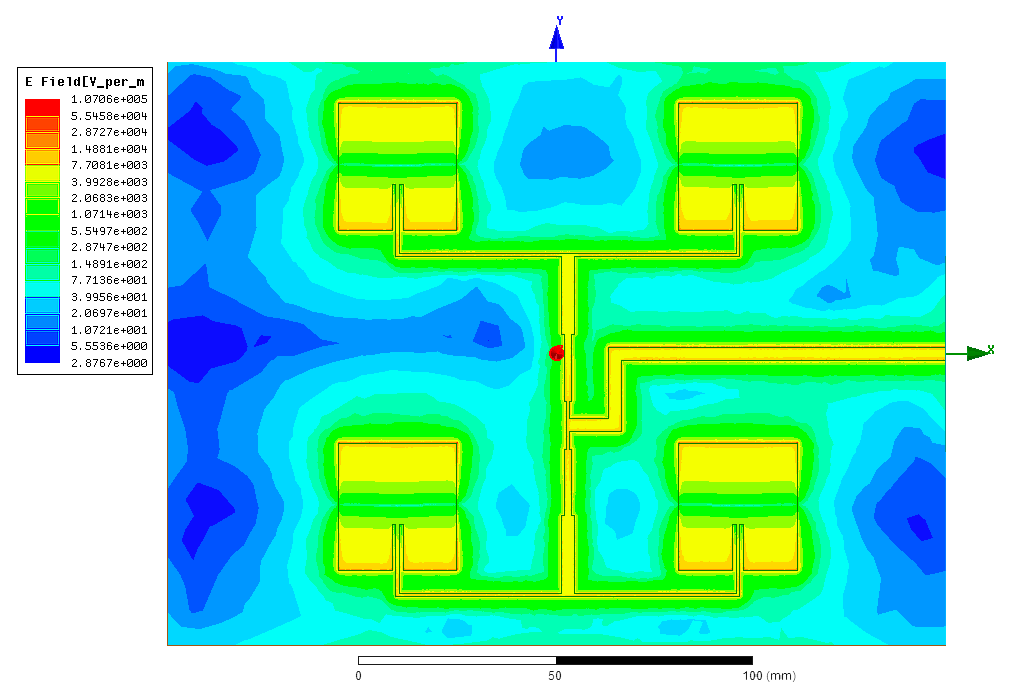
\includegraphics[width=\textwidth]{archivos/analisis/2x21/8}
        \caption{Distribución de campos eléctricos para el para el array 2x2 a 2.4 GHz}
        \label{fig:elec2x21}
\end{figure}

\subsection{Resumen}
\par En la configuración 2x2 a 2.4 GHz se puede observar una pérdida de la eficiencia de radiación de la antena, así como un menor ancho de banda, aunque dentro del mismo rango de las antenas cuya frecuencia de trabajo es de 2.4 GHz, como se irá comprobando a lo largo del análisis. También ha llegado a empeorar la relación delante atrás, lo que puede suponer interferencias no deseadas con otras antenas. Por otro lado, el patrón de directividad es simétrico y con lóbulos laterales controlados.
\\
\par En la tabla \ref{tab:res2x21} se pueden observar un resumen de los parámetros característicos de la antena.

\begin{table}[H]
  
   
   \small % text size of table content
   \centering % center the table
   \begin{tabular}{c c} % alignment of each column data
   \toprule[\heavyrulewidth]\toprule[\heavyrulewidth]
   \textbf{Parámetro} & \textbf{Array 2x2 a 2.4 GHz} \\ 
   \midrule
   \textbf{$S_{11}$} & -40.70 dB \\
   \textbf{Ancho de banda} & 34.6 MHz \\
   \textbf{Directividad} & 10.74 dB \\
   \textbf{Ganancia} & 9.98 dB \\
   \textbf{Eficiencia de radiación} & 83.81\% \\
   \textbf{Relación delante/atrás} & 19.56 dB \\

   \bottomrule[\heavyrulewidth] 
   \end{tabular}
   
   \caption{Parámetros característicos del array 2x2 a 2.4 GHz} 
   \label{tab:res2x21}
\end{table}












\section{Array 2x2 a 6 GHz}
\par Para el array en configuración 2x2 a 6 GHz los resultados obtenidos son los siguientes:

\subsection{Pérdidas de retorno}
\par En cuanto a su curva de pérdidas de retorno del array a 6 GHz, se puede observar un valor pico de -35.76 dB y un ancho de banda de 162.5 MHz, desde los 6.078 GHz hasta los 5.915 GHz, lo que equivale a un 2.7\% de la frecuencia de trabajo.
\\
\begin{figure}[H]
    \centering
        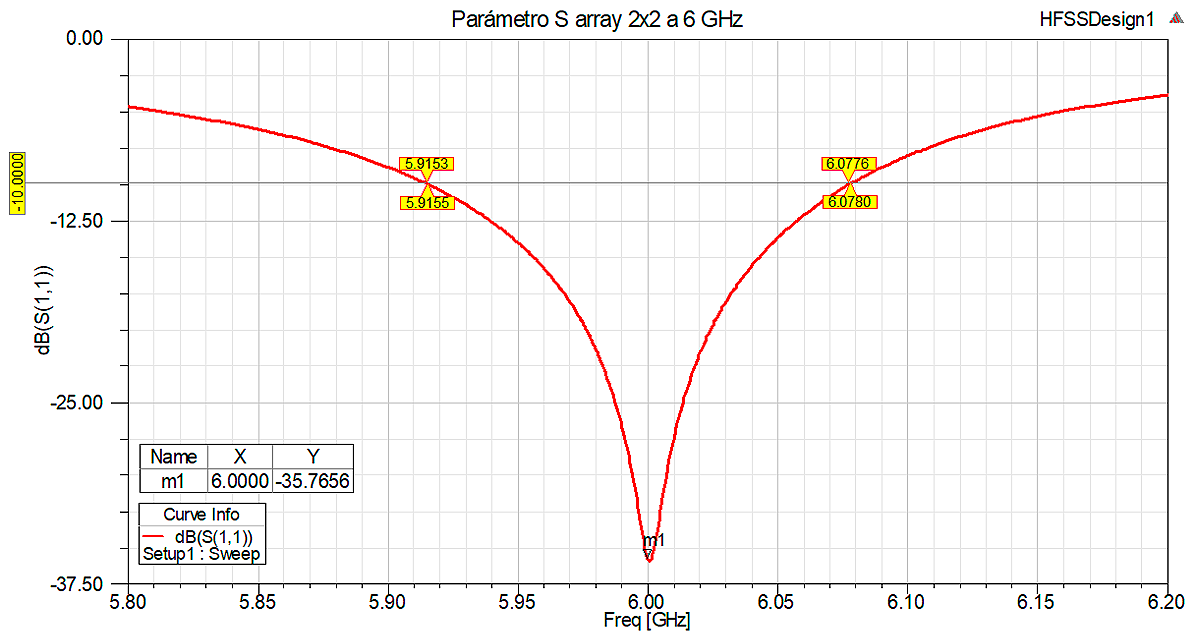
\includegraphics[width=\textwidth]{archivos/analisis/2x22/1}
        \caption{Parámetro $S_{11}$ para el array 2x2 a 6 GHz}
        \label{fig:s2x22}
\end{figure}

\newpage
\subsection{Reactancia}
\par La curva de reactancia arroja un valor a la frecuencia de trabajo de -1.57 $\Omega$. 
\\
\begin{figure}[H]
    \centering
        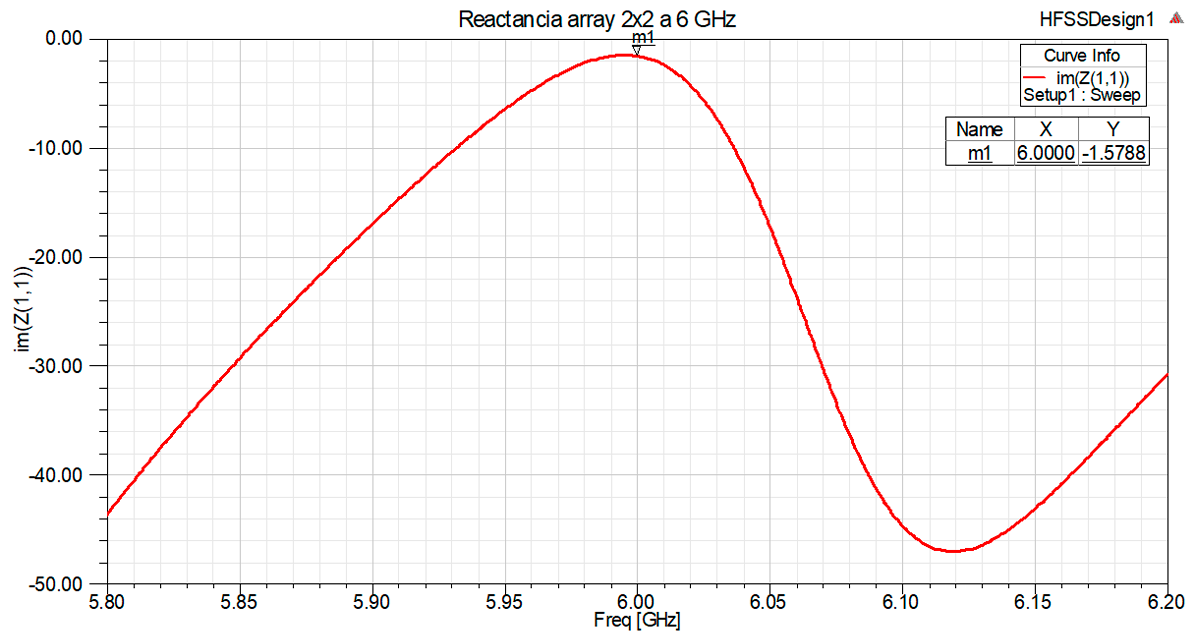
\includegraphics[width=0.8\textwidth]{archivos/analisis/2x22/2}
        \caption{Reactancia para el array 2x2 a 6 GHz}
        \label{fig:react2x22}
\end{figure}

\subsection{Resistencia}
\par La parte real de la impedancia ofrece un valor a la frecuencia de trabajo de 49.62 $\Omega$.
\\
\begin{figure}[H]
    \centering
        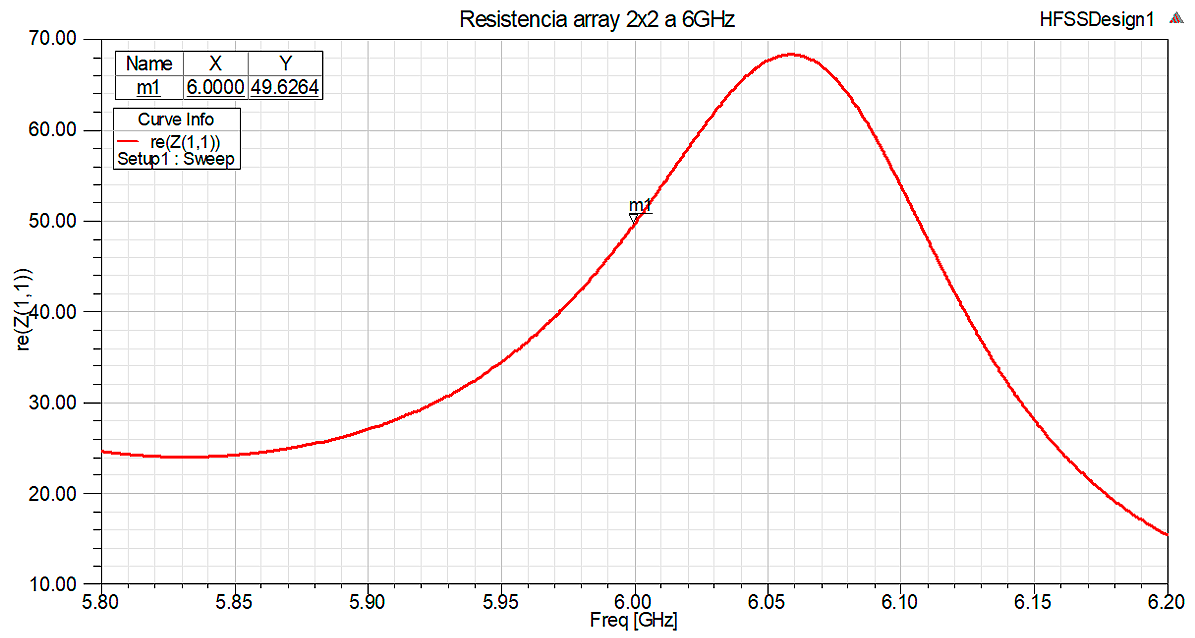
\includegraphics[width=0.8\textwidth]{archivos/analisis/2x22/3}
        \caption{Resistencia para el array 2x2 a 6 GHz}
        \label{fig:resis2x22}
\end{figure}

\subsection{Patrón de radiación}
\par El patrón de directividad que encontramos en el array 2x2 a 6 GHz difiere mucho del que encontramos en la misma configuración a 2.4 GHz. Se puede comprobar un amento de 2 dB de directividad hasta los 12.88 dB, así como comportamientos asimetricos en ambos planos de radiación. 
\\
\subsubsection{Plano E}
\begin{figure}[H]
    \centering
        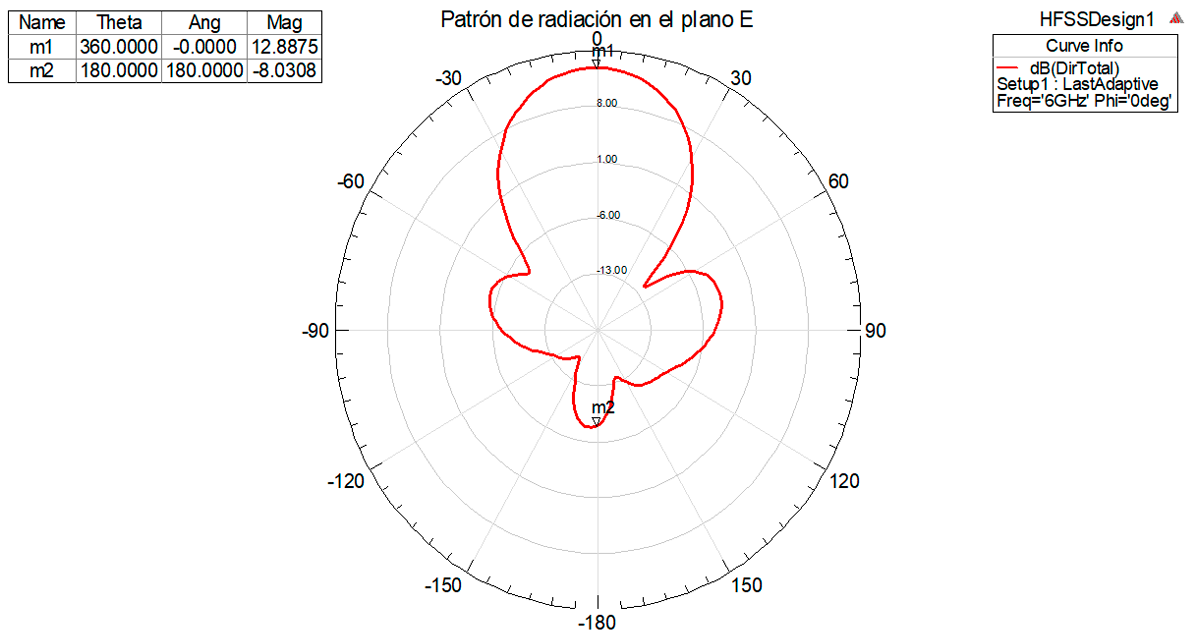
\includegraphics[width=0.8\textwidth]{archivos/analisis/2x22/4}
        \caption{Radiación en el plano E para el array 2x2 a 6 GHz}
        \label{fig:E2x22}
\end{figure}

\subsubsection{Plano H}
\begin{figure}[H]
    \centering
        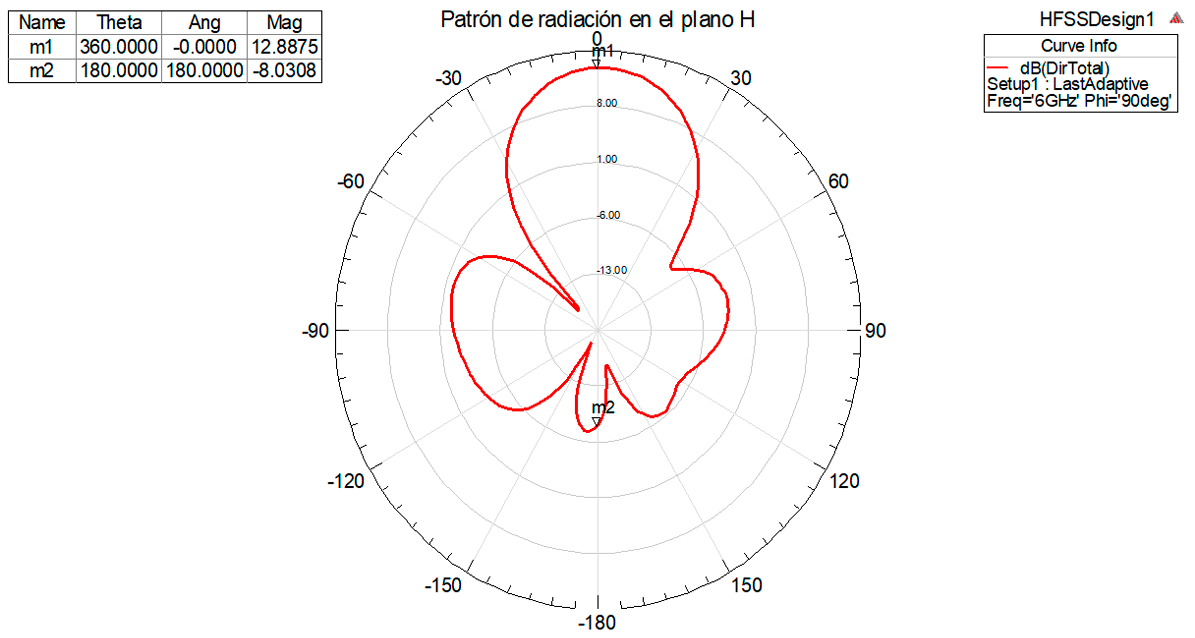
\includegraphics[width=0.8\textwidth]{archivos/analisis/2x22/5}
        \caption{Radiación en el plano H para el array 2x2 a 6 GHz}
        \label{fig:H2x22}
\end{figure}

\subsection{Radiación 3D}
\par En el diagrama de radiación 3D se puede comprobar el resultado del comportamiento asimétrico en los dos planos de radiación. Aunque la base del patrón intente ser la misma que la encontrada en la configuración a 2.4 GHz, se hacen notables ciertas deformidades en el lóbulo principal así como en algunos de los lóbulos secundarios.

\begin{figure}[H]
     \centering
     \begin{subfigure}[b]{0.7\textwidth}
         \centering
         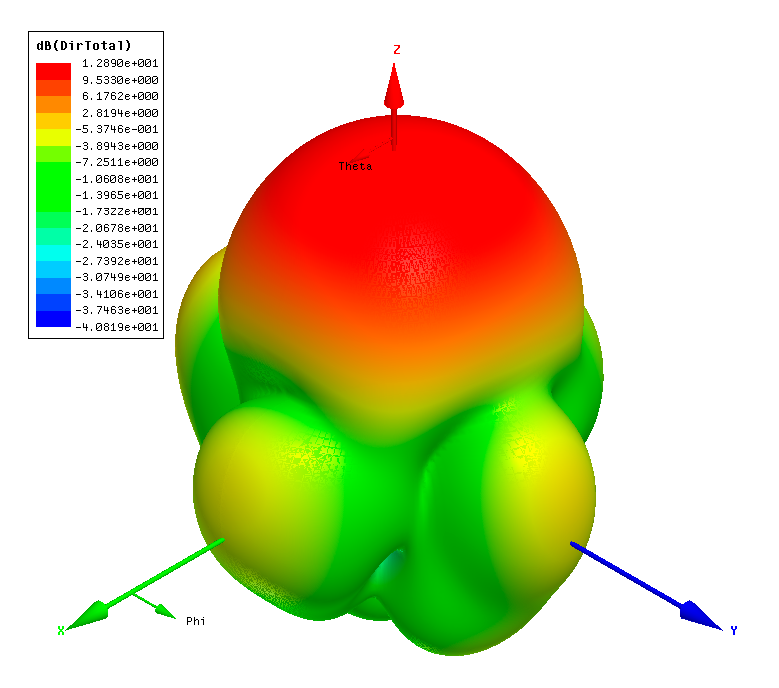
\includegraphics[width=0.85\textwidth]{archivos/analisis/2x22/6}
         \caption{Representación isométrica del diagrama de radiación 3D}
         \label{fig:3d12x22}
     \end{subfigure}
     \hfill
     \begin{subfigure}[b]{0.7\textwidth}
         \centering
         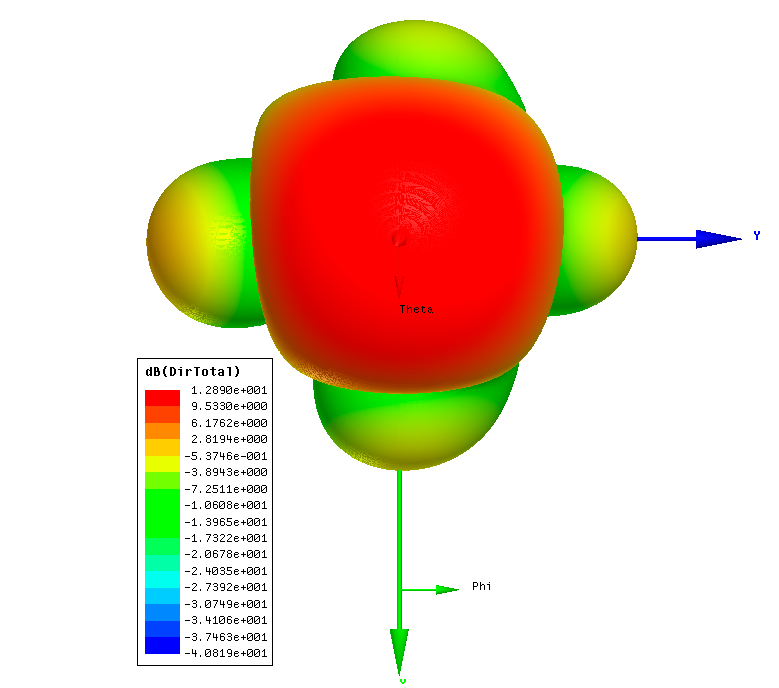
\includegraphics[width=0.85\textwidth]{archivos/analisis/2x22/7}
         \caption{Representación superior del diagrama de radiación 3D}
         \label{fig:3d22x22}
     \end{subfigure}
     \hfill
        \caption{Radiación 3D para el array 2x2 a 6 GHz}
        \label{fig:3d2x22}
\end{figure}

\subsection{Campo eléctrico}
\par Finalmente, podemos observar la distribución de campos eléctricos en el parche. 

\begin{figure}[H]
    \centering
        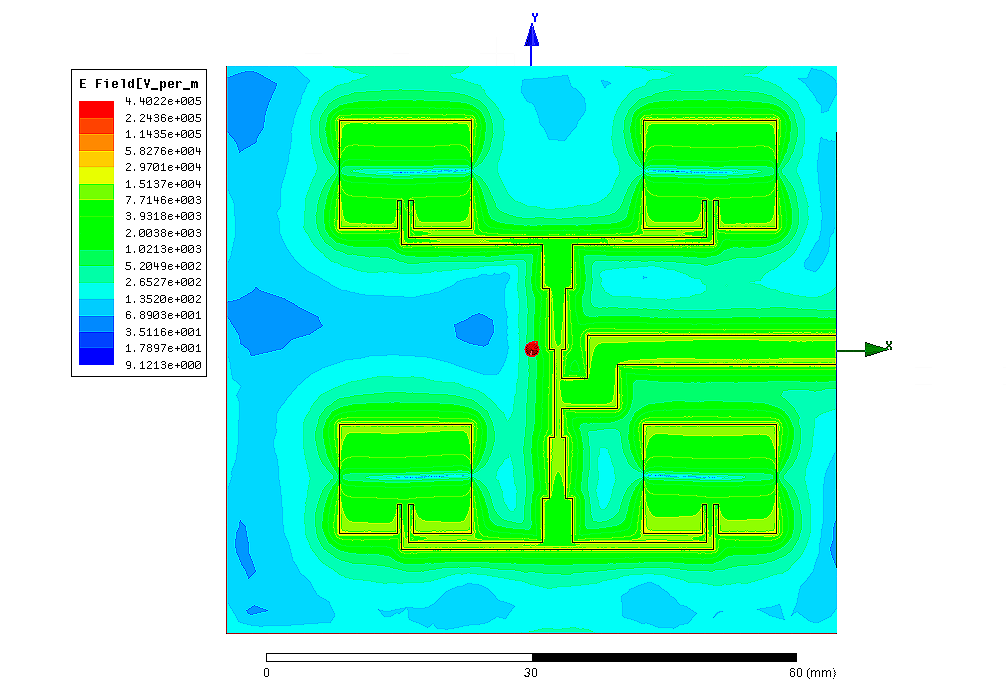
\includegraphics[width=\textwidth]{archivos/analisis/2x22/8}
        \caption{Distribución de campos eléctricos para el para el array 2x2 a 6 GHz}
        \label{fig:elec2x22}
\end{figure}

\subsection{Resumen}
\par La principal razón por la que se haya podido producir estos patrones no simétricos en esta configuración es el hecho de que la proximidad entre los parches y las líneas de transmisión que alimentan al array hayan afectado a la propagación de las ondas. Aun así la eficiencia de esta antena ronda el 90\% \todo{no puedo ver el comentario} con lo que la adaptación entre las líneas y la antena ha sido buena y la directividad ha aumentado considerablemente respecto a la antena de 2.4 GHz.
\\
\par En la tabla \ref{tab:res2x22} se pueden observar un resumen de los parámetros característicos de la antena.

\begin{table}[H]
  
   
   \small % text size of table content
   \centering % center the table
   \begin{tabular}{c c} % alignment of each column data
   \toprule[\heavyrulewidth]\toprule[\heavyrulewidth]
   \textbf{Parámetro} & \textbf{Array 2x2 a 6 GHz} \\ 
   \midrule
   \textbf{$S_{11}$} & -35.76 dB \\
   \textbf{Ancho de banda} & 162.5 MHz \\
   \textbf{Directividad} & 12.88 dB \\
   \textbf{Ganancia} & 12.47 dB \\
   \textbf{Eficiencia de radiación} & 90.8\% \\
   \textbf{Relación delante/atrás} & 20.7 dB \\

   \bottomrule[\heavyrulewidth] 
   \end{tabular}
   
   \caption{Parámetros característicos del array 2x2 a 6 GHz} 
   \label{tab:res2x22}
\end{table}




















\section{Array 4x1 a 2.4 GHz}
\par Para el array en configuración 4x1 a 2.4 GHz los resultados obtenidos son los siguientes:

\subsection{Pérdidas de retorno}
\par En cuanto a su curva de pérdidas de retorno del array 4x1 a 2.4 GHz, se puede observar un valor pico de -57.12 dB y un ancho de banda de 41.1 MHz, desde los 2.3799 GHz hasta los 2.421 GHz, lo que equivale a un 1.71\% de la frecuencia de trabajo.
\\
\begin{figure}[H]
    \centering
        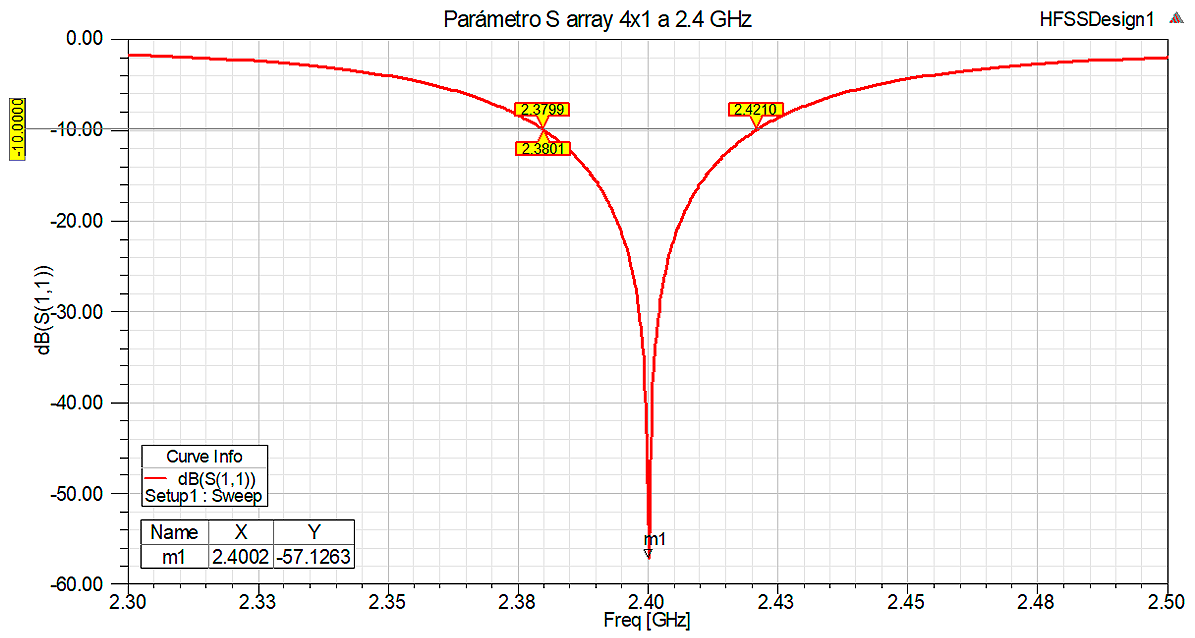
\includegraphics[width=\textwidth]{archivos/analisis/4x11/1}
        \caption{Parámetro $S_{11}$ para el array 4x1 a 2.4 GHz}
        \label{fig:s4x11}
\end{figure}

\newpage
\subsection{Reactancia}
\par La curva de reactancia arroja un valor a la frecuencia de trabajo de -0.11 $\Omega$. 
\\
\begin{figure}[H]
    \centering
        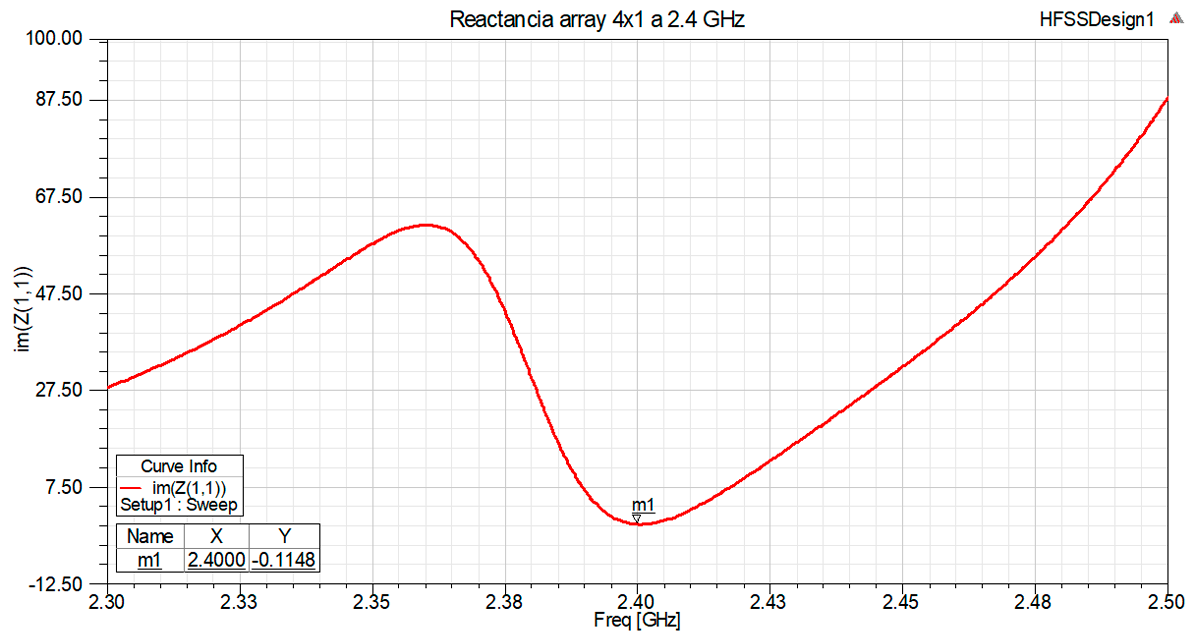
\includegraphics[width=0.8\textwidth]{archivos/analisis/4x11/2}
        \caption{Reactancia para el array 4x1 a 2.4 GHz}
        \label{fig:react4x11}
\end{figure}

\subsection{Resistencia}
\par La parte real de la impedancia ofrece un valor a la frecuencia de trabajo de 50.26 $\Omega$.
\\
\begin{figure}[H]
    \centering
        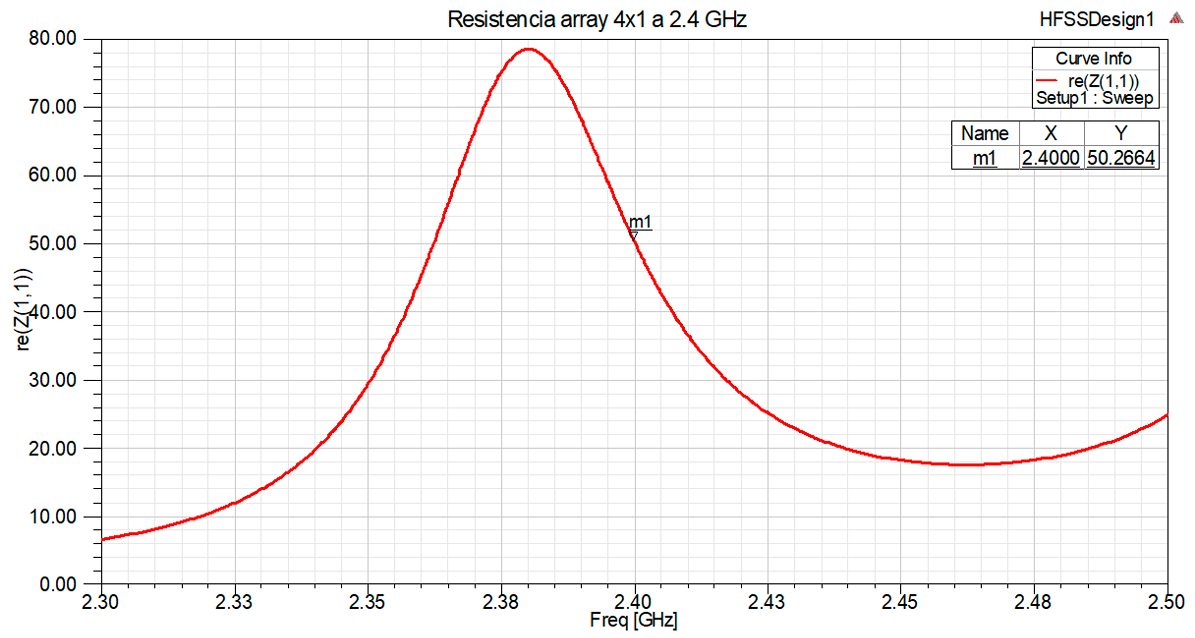
\includegraphics[width=0.8\textwidth]{archivos/analisis/4x11/3}
        \caption{Resistencia para el array 4x1 a 2.4 GHz}
        \label{fig:resis4x11}
\end{figure}

\subsection{Patrón de radiación}
\par En este nuevo tipo de configuración donde se han añadido más parches se puede comprobar el aumento de complejidad del patrón de radiación, donde han aparecido más lóbulos laterales y traseros en el plano E. En el plano H encontramos un patrón omnidireccional. La directividad en el ángulo de máxima radiación es de 11.6 dB.
\\
\subsubsection{Plano E}
\begin{figure}[H]
    \centering
        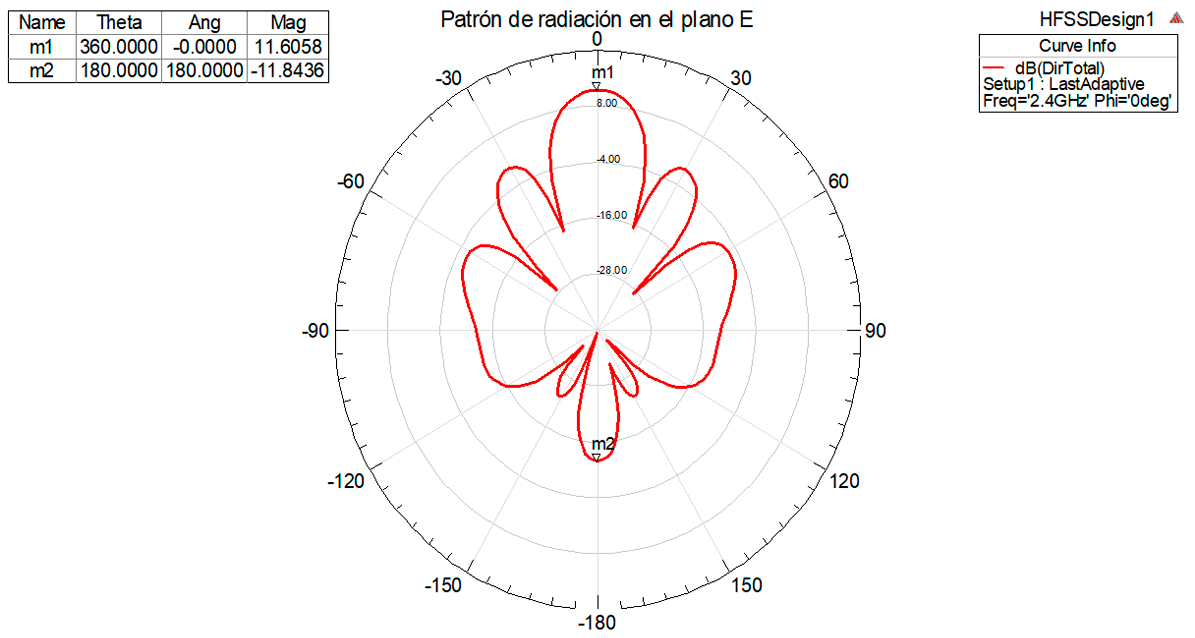
\includegraphics[width=0.8\textwidth]{archivos/analisis/4x11/4}
        \caption{Radiación en el plano E para el array 4x1 a 2.4 GHz}
        \label{fig:E4x11}
\end{figure}

\subsubsection{Plano H}
\begin{figure}[H]
    \centering
        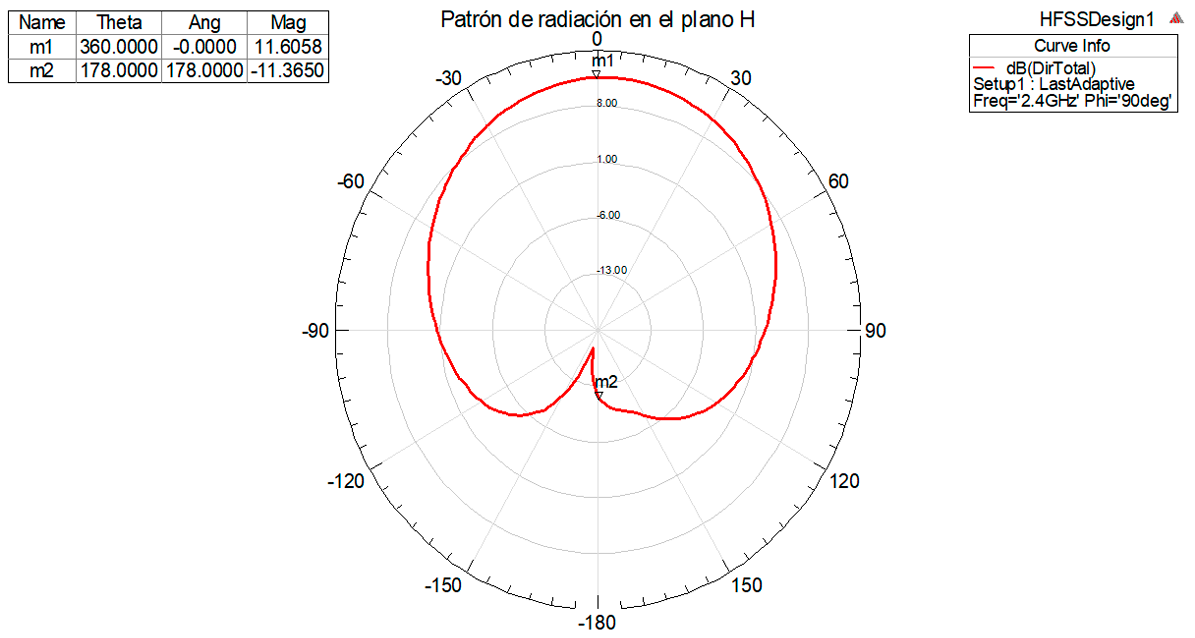
\includegraphics[width=0.8\textwidth]{archivos/analisis/4x11/5}
        \caption{Radiación en el plano H para el array 4x1 a 2.4 GHz}
        \label{fig:H4x11}
\end{figure}

\subsection{Radiación 3D}
\par Con el diagrama de radiación 3D se puede observar un comportamiento muy parecido al que obteníamos con las antenas en configuración 2x1, pero el aumento de parches ha ofrecido al patrón de radiación una mayor directividad así como complejidad y la presencia de elementos que quizás no sean deseados.

\begin{figure}[H]
     \centering
     \begin{subfigure}[b]{0.7\textwidth}
         \centering
         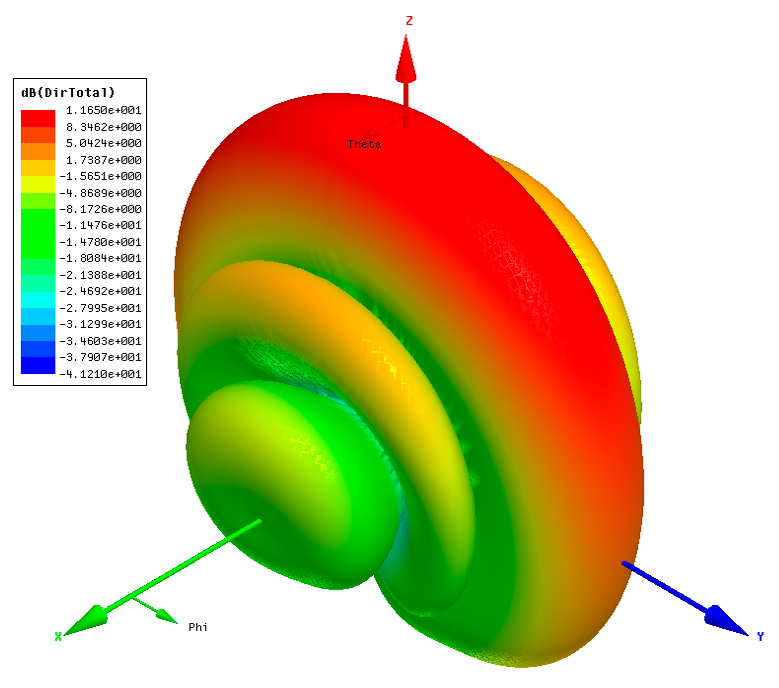
\includegraphics[width=0.85\textwidth]{archivos/analisis/4x11/6}
         \caption{Representación isométrica del diagrama de radiación 3D}
         \label{fig:3d14x11}
     \end{subfigure}
     \hfill
     \begin{subfigure}[b]{0.7\textwidth}
         \centering
         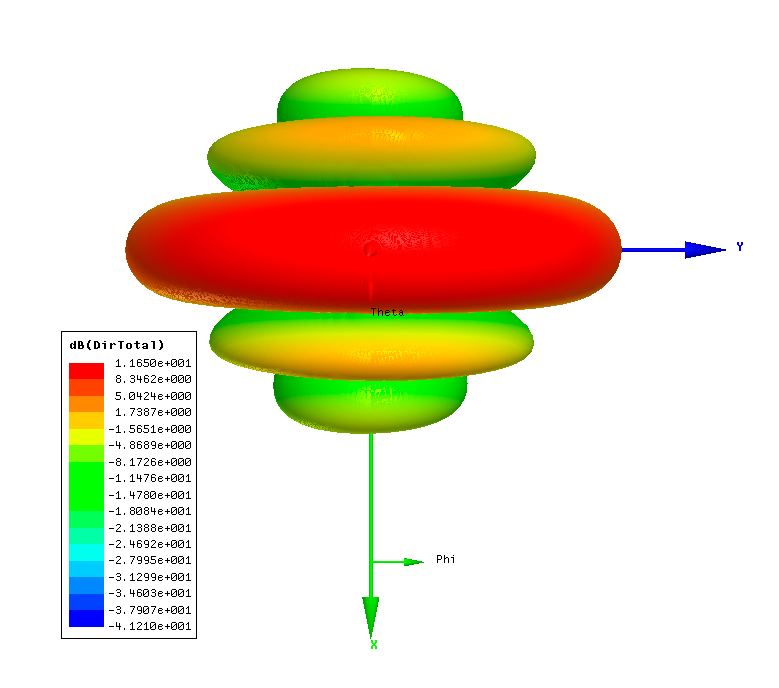
\includegraphics[width=0.85\textwidth]{archivos/analisis/4x11/7}
         \caption{Representación superior del diagrama de radiación 3D}
         \label{fig:3d24x11}
     \end{subfigure}
     \hfill
        \caption{Radiación 3D para el array 4x1 a 2.4 GHz}
        \label{fig:3d4x11}
\end{figure}

\subsection{Campo eléctrico}
\par Finalmente, podemos observar la distribución de campos eléctricos en el parche. 

\begin{figure}[H]
    \centering
        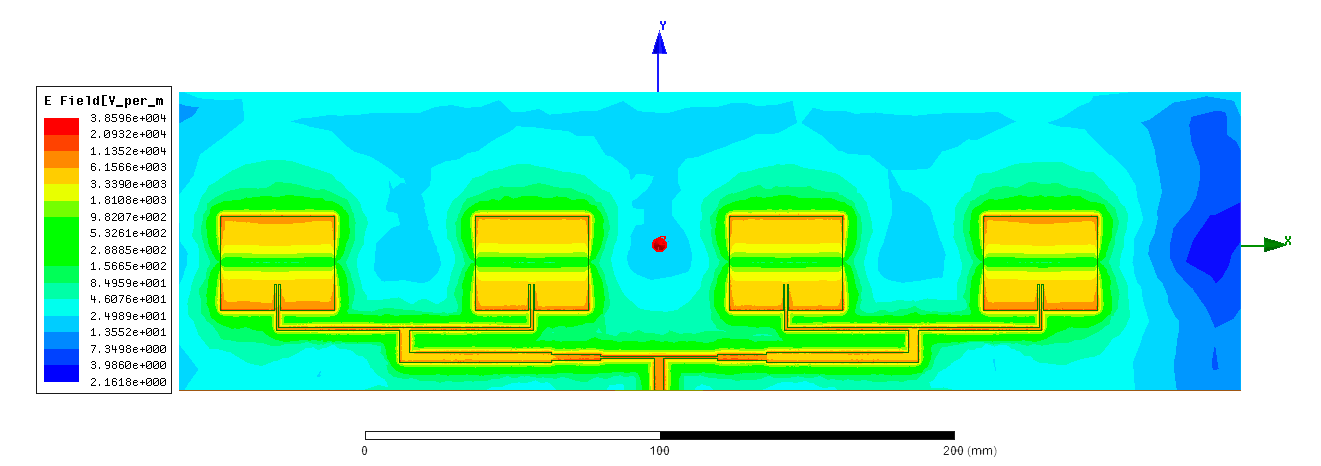
\includegraphics[width=\textwidth]{archivos/analisis/4x11/8}
        \caption{Distribución de campos eléctricos para el para el array 4x1 a 2.4 GHz}
        \label{fig:elec4x11}
\end{figure}

\subsection{Resumen}
\par Aunque la eficiencia de esta configuración haya disminuido, los valores obtenidos entran dentro de los margenes de buen funcionamiento y el patrón de directividad obtenido puede ser muy útil para aplicaciones de telefonía móvil, como se explicó en el array 2x1. Poco a poco va aumentando la directividad de nuestros arrays debido a la inclusión de una mayor número de parches, pero esto trae consigo la obtención de patrones de directividad más complejos con mayor número de lóbulos secundarios y traseros. 
\\
\par En la tabla \ref{tab:res4x11} se pueden observar un resumen de los parámetros característicos de la antena.

\begin{table}[H]
  
   
   \small % text size of table content
   \centering % center the table
   \begin{tabular}{c c} % alignment of each column data
   \toprule[\heavyrulewidth]\toprule[\heavyrulewidth]
   \textbf{Parámetro} & \textbf{Array 4x1 a 2.4 GHz} \\ 
   \midrule
   \textbf{$S_{11}$} & -57.12 dB \\
   \textbf{Ancho de banda} & 41.4 MHz \\
   \textbf{Directividad} & 11.6 dB \\
   \textbf{Ganancia} & 11.04 dB \\
   \textbf{Eficiencia de radiación} & 86.97\% \\
   \textbf{Relación delante/atrás} & 24.74 dB \\

   \bottomrule[\heavyrulewidth] 
   \end{tabular}
   
   \caption{Parámetros característicos del array 4x1 a 2.4 GHz} 
   \label{tab:res4x11}
\end{table}




















\newpage
\section{Array 4x1 a 6 GHz}
\par Para el array en configuración 4x1 a 6 GHz los resultados obtenidos son los siguientes:

\subsection{Pérdidas de retorno}
\par En cuanto a su curva de pérdidas de retorno del array 4x1 a 6 GHz, se puede observar un valor pico de -30.97 dB y un ancho de banda de 223.8 MHz, desde los 5.8674 GHz hasta los 6.0912 GHz, lo que equivale a un 3.73\% de la frecuencia de trabajo.
\\
\begin{figure}[H]
    \centering
        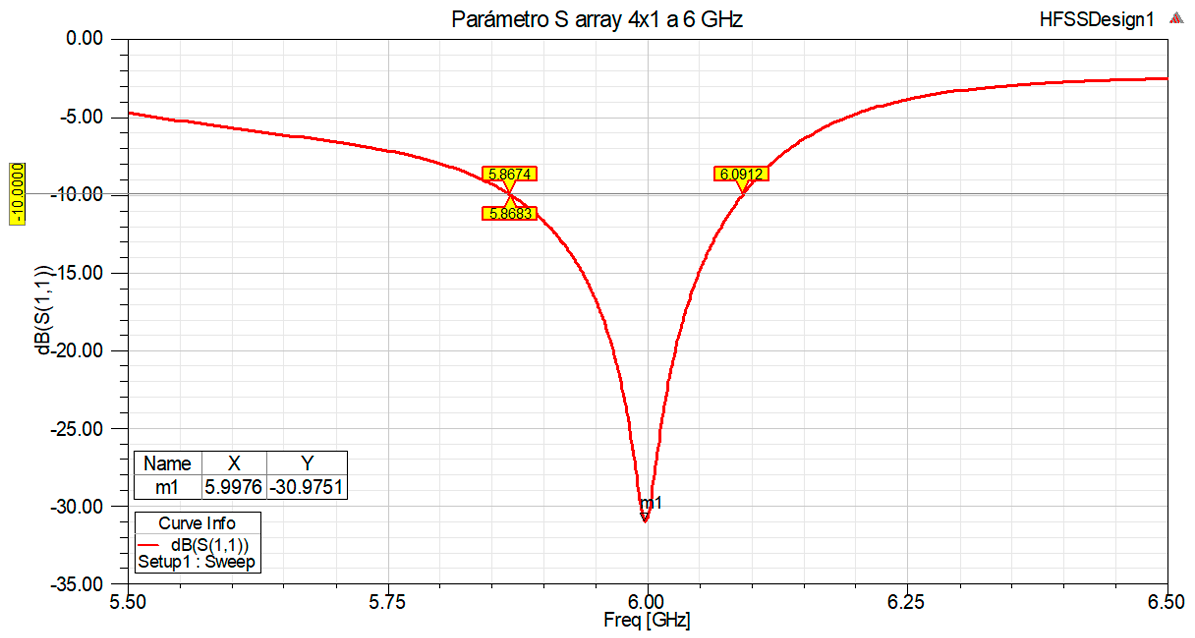
\includegraphics[width=\textwidth]{archivos/analisis/4x12/1}
        \caption{Parámetro $S_{11}$ para el array 4x1 a 6 GHz}
        \label{fig:s4x12}
\end{figure}

\newpage
\subsection{Reactancia}
\par La curva de reactancia arroja un valor a la frecuencia de trabajo de -0.6 $\Omega$. 
\\
\begin{figure}[H]
    \centering
        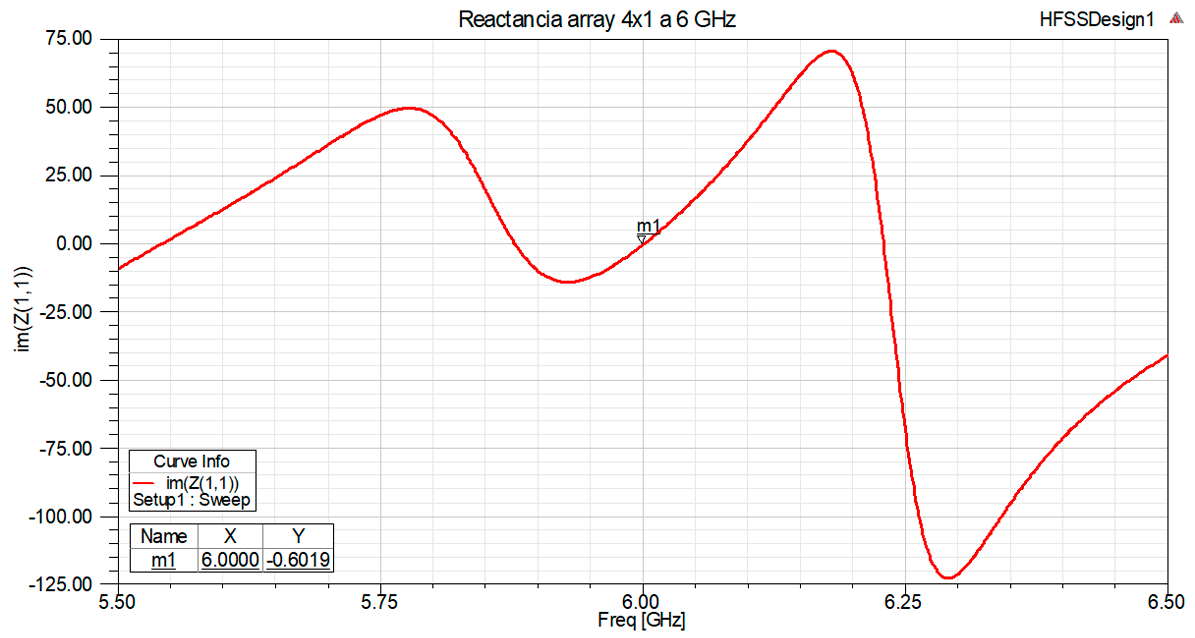
\includegraphics[width=0.8\textwidth]{archivos/analisis/4x12/2}
        \caption{Reactancia para el array 4x1 a 6 GHz}
        \label{fig:react4x12}
\end{figure}

\subsection{Resistencia}
\par La parte real de la impedancia ofrece un valor a la frecuencia de trabajo de 47.21 $\Omega$.
\\
\begin{figure}[H]
    \centering
        \includegraphics[width=0.8\textwidth]{archivos/analisis/4x12/3}
        \caption{Resistencia para el array 4x1 a 6 GHz}
        \label{fig:resis4x12}
\end{figure}

\subsection{Patrón de radiación}
\par El patrón de directividad de esta configuración es bastante parecido al obtenido en la configuración a 2.4 GHz, con la diferencia de que encontramos nulos menos definidos. También, como veremos, el lóbulo trasero aumenta de directividad, lo que significa una reducción de la relación delante/atrás.
\\
\subsubsection{Plano E}
\begin{figure}[H]
    \centering
        \includegraphics[width=0.8\textwidth]{archivos/analisis/4x12/4}
        \caption{Radiación en el plano E para el array 4x1 a 6 GHz}
        \label{fig:E4x12}
\end{figure}

\subsubsection{Plano H}
\begin{figure}[H]
    \centering
        \includegraphics[width=0.8\textwidth]{archivos/analisis/4x12/5}
        \caption{Radiación en el plano H para el array 4x1 a 6 GHz}
        \label{fig:H4x12}
\end{figure}

\subsection{Radiación 3D}
\par El diagrama de radiación 3D presenta una forma muy similar a la encontrada en el array de la misma configuración a 2.4 GHz, aunque con pequeñas diferencias de forma en los lóbulos laterales.

\begin{figure}[H]
     \centering
     \begin{subfigure}[b]{0.7\textwidth}
         \centering
         \includegraphics[width=0.85\textwidth]{archivos/analisis/4x12/6}
         \caption{Representación isométrica del diagrama de radiación 3D}
         \label{fig:3d14x12}
     \end{subfigure}
     \hfill
     \begin{subfigure}[b]{0.7\textwidth}
         \centering
         \includegraphics[width=0.85\textwidth]{archivos/analisis/4x12/7}
         \caption{Representación superior del diagrama de radiación 3D}
         \label{fig:3d24x12}
     \end{subfigure}
     \hfill
        \caption{Radiación 3D para el array 4x1 a 6 GHz}
        \label{fig:3d4x12}
\end{figure}

\subsection{Campo eléctrico}
\par Finalmente, podemos observar la distribución de campos eléctricos en el parche. 

\begin{figure}[H]
    \centering
        \includegraphics[width=\textwidth]{archivos/analisis/4x12/8}
        \caption{Distribución de campos eléctricos para el para el array 4x1 a 6 GHz}
        \label{fig:elec4x12}
\end{figure}

\subsection{Resumen}
\par Aunque la adaptación de la antena no haya sido de las mejores obtenidas, como se puede observar en el valor de pérdidas de retorno S, esta antena ha obtenido unos parámetros de funcionamiento excepcionales en cuanto a directividad, eficiencia y ancho de banda. Se ha llegado a obtener hasta 200 MHz de ancho de banda, lo que supone un 3.73\% sobre la frecuencia de trabajo, rozando el límite de ancho de banda que se puede llegar a obtener en una configuración de alimentación por conexión directa de línea microstrip.
\\
\par En la tabla \ref{tab:res4x12} se pueden observar un resumen de los parámetros característicos de la antena.

\begin{table}[H]
  
   
   \small % text size of table content
   \centering % center the table
   \begin{tabular}{c c} % alignment of each column data
   \toprule[\heavyrulewidth]\toprule[\heavyrulewidth]
   \textbf{Parámetro} & \textbf{Array 4x1 a 6 GHz} \\ 
   \midrule
   \textbf{$S_{11}$} & -30.97 dB \\
   \textbf{Ancho de banda} & 223.8 MHz \\
   \textbf{Directividad} & 12.56 dB \\
   \textbf{Ganancia} & 12.16 dB \\
   \textbf{Eficiencia de radiación} & 91.3\% \\
   \textbf{Relación delante/atrás} & 24.3 dB \\

   \bottomrule[\heavyrulewidth] 
   \end{tabular}
   
   \caption{Parámetros característicos del array 4x1 a 6 GHz} 
   \label{tab:res4x12}
\end{table}























\newpage
\section{Array 4x2 a 2.4 GHz}
\par Para el array en configuración 4x2 a 2.4 GHz los resultados obtenidos son los siguientes:

\subsection{Pérdidas de retorno}
\par En cuanto a su curva de pérdidas de retorno del array 4x2 a 2.4 GHz, se puede observar un valor pico de -32.18 dB y un ancho de banda de 39.6 MHz, desde los 2.3792 GHz hasta los 2.4186 GHz, lo que equivale a un 1.65\% de la frecuencia de trabajo.
\\
\begin{figure}[H]
    \centering
        \includegraphics[width=\textwidth]{archivos/analisis/4x21/1}
        \caption{Parámetro $S_{11}$ para el array 4x2 a 2.4 GHz}
        \label{fig:s4x21}
\end{figure}

\newpage
\subsection{Reactancia}
\par La curva de reactancia arroja un valor a la frecuencia de trabajo de -1.39 $\Omega$. 
\\
\begin{figure}[H]
    \centering
        \includegraphics[width=0.8\textwidth]{archivos/analisis/4x21/2}
        \caption{Reactancia para el array 4x2 a 2.4 GHz}
        \label{fig:react4x21}
\end{figure}

\subsection{Resistencia}
\par La parte real de la impedancia ofrece un valor a la frecuencia de trabajo de 52.07 $\Omega$.
\\
\begin{figure}[H]
    \centering
        \includegraphics[width=0.8\textwidth]{archivos/analisis/4x21/3}
        \caption{Resistencia para el array 4x2 a 2.4 GHz}
        \label{fig:resis4x21}
\end{figure}

\subsection{Patrón de radiación}
\par Al duplicar la fila que se poseía en el array 4x1 se ha obtenido el mismo patrón de directividad que esta en el plano E, pero con una mayor área de radiación en los lóbulos laterales, aumentando de cobertura en estas zonas. La directividad obtenida en el ángulo de máxima radiación es de 13.97 dB. En el plano H vemos un patrón casi omnidireccional, como ocurría en el array 4x1 pero con ciertos nulos creando lóbulos laterales más definidos.
\\
\subsubsection{Plano E}
\begin{figure}[H]
    \centering
        \includegraphics[width=0.75\textwidth]{archivos/analisis/4x21/4}
        \caption{Radiación en el plano E para el array 4x2 a 2.4 GHz}
        \label{fig:E4x21}
\end{figure}

\subsubsection{Plano H}
\begin{figure}[H]
    \centering
        \includegraphics[width=0.75\textwidth]{archivos/analisis/4x21/5}
        \caption{Radiación en el plano H para el array 4x2 a 2.4 GHz}
        \label{fig:H4x21}
\end{figure}

\subsection{Radiación 3D}
\par La conjunción de ambos planos de radiación lleva a la obtención de un diagrama de radiación 3D muy complejo con un gran número de lóbulos laterales y secundarios a costa de conseguir una de las directividades más altas logradas hasta el momento en el proyecto.

\begin{figure}[H]
     \centering
     \begin{subfigure}[b]{0.7\textwidth}
         \centering
         \includegraphics[width=0.85\textwidth]{archivos/analisis/4x21/6}
         \caption{Representación isométrica del diagrama de radiación 3D}
         \label{fig:3d14x21}
     \end{subfigure}
     \hfill
     \begin{subfigure}[b]{0.7\textwidth}
         \centering
         \includegraphics[width=0.85\textwidth]{archivos/analisis/4x21/7}
         \caption{Representación superior del diagrama de radiación 3D}
         \label{fig:3d24x21}
     \end{subfigure}
     \hfill
        \caption{Radiación 3D para el array 4x2 a 2.4 GHz}
        \label{fig:3d4x21}
\end{figure}

\subsection{Campo eléctrico}
\par Finalmente, podemos observar la distribución de campos eléctricos en el parche. 

\begin{figure}[H]
    \centering
        \includegraphics[width=\textwidth]{archivos/analisis/4x21/8}
        \caption{Distribución de campos eléctricos para el para el array 4x2 a 2.4 GHz}
        \label{fig:elec4x21}
\end{figure}

\subsection{Resumen}
\par Esta configuración es una de las que mas ha costado conseguir adaptar en el proceso de diseño, es por ello que los resultados obtenidos no destacan sobre el resto de arrays. La directividad obtenida ha sido muy buena, pero otros parámetros como la eficiencia o el ancho de banda han dejado que desear sobre esta configuración. 
\\
\par En la tabla \ref{tab:res4x21} se pueden observar un resumen de los parámetros característicos de la antena.

\begin{table}[H]
  
   
   \small % text size of table content
   \centering % center the table
   \begin{tabular}{c c} % alignment of each column data
   \toprule[\heavyrulewidth]\toprule[\heavyrulewidth]
   \textbf{Parámetro} & \textbf{Array 4x2 a 2.4 GHz} \\ 
   \midrule
   \textbf{$S_{11}$} & -32.18 dB \\
   \textbf{Ancho de banda} & 39.6 MHz \\
   \textbf{Directividad} & 13.97 dB \\
   \textbf{Ganancia} & 13.17 dB \\
   \textbf{Eficiencia de radiación} & 83.08\% \\
   \textbf{Relación delante/atrás} & 25.15 dB \\

   \bottomrule[\heavyrulewidth] 
   \end{tabular}
   
   \caption{Parámetros característicos del array 4x2 a 2.4 GHz} 
   \label{tab:res4x21}
\end{table}





















\newpage
\section{Array 4x2 a 6 GHz}
\par Para el array en configuración 4x2 a 6 GHz los resultados obtenidos son los siguientes:

\subsection{Pérdidas de retorno}
\par En cuanto a su curva de pérdidas de retorno del array 4x2 a 6 GHz, se puede observar un valor pico de -12.02 dB y un ancho de banda de 46.9 MHz, desde los 5.9757 GHz hasta los 6.0226 GHz, lo que equivale a un 0.78\% de la frecuencia de trabajo.
\\
\begin{figure}[H]
    \centering
        \includegraphics[width=\textwidth]{archivos/analisis/4x22/1}
        \caption{Parámetro $S_{11}$ para el array 4x2 a 6 GHz}
        \label{fig:s4x22}
\end{figure}

\newpage
\subsection{Reactancia}
\par La curva de reactancia arroja un valor a la frecuencia de trabajo de -7.41 $\Omega$. 
\\
\begin{figure}[H]
    \centering
        \includegraphics[width=0.8\textwidth]{archivos/analisis/4x22/2}
        \caption{Reactancia para el array 4x2 a 6 GHz}
        \label{fig:react4x22}
\end{figure}

\subsection{Resistencia}
\par La parte real de la impedancia ofrece un valor a la frecuencia de trabajo de 82.36 $\Omega$.
\\
\begin{figure}[H]
    \centering
        \includegraphics[width=0.8\textwidth]{archivos/analisis/4x22/3}
        \caption{Resistencia para el array 4x2 a 6 GHz}
        \label{fig:resis4x22}
\end{figure}

\subsection{Patrón de radiación}
\par Al duplicar la fila que se poseía en el array 4x1 se ha obtenido el mismo patrón de directividad que esta en el plano E, pero con una mayor área de radiación en los lóbulos laterales, aumentando de cobertura en estas zonas. La directividad obtenida en el ángulo de máxima radiación es de 13.97 dB. En el plano H vemos un patrón casi omnidireccional, como ocurría en el array 4x1 pero con ciertos nulos creando lóbulos laterales más definidos.
\\
\subsubsection{Plano E}
\begin{figure}[H]
    \centering
        \includegraphics[width=0.75\textwidth]{archivos/analisis/4x22/4}
        \caption{Radiación en el plano E para el array 4x2 a 6 GHz}
        \label{fig:E4x22}
\end{figure}

\subsubsection{Plano H}
\begin{figure}[H]
    \centering
        \includegraphics[width=0.75\textwidth]{archivos/analisis/4x22/5}
        \caption{Radiación en el plano H para el array 4x2 a 6 GHz}
        \label{fig:H4x22}
\end{figure}

\subsection{Radiación 3D}
\par La conjunción de ambos planos de radiación lleva a la obtención de un diagrama de radiación 3D muy complejo con un gran número de lóbulos laterales y secundarios a costa de conseguir una de las directividades más altas logradas hasta el momento en el proyecto.

\begin{figure}[H]
     \centering
     \begin{subfigure}[b]{0.7\textwidth}
         \centering
         \includegraphics[width=0.85\textwidth]{archivos/analisis/4x22/6}
         \caption{Representación isométrica del diagrama de radiación 3D}
         \label{fig:3d14x22}
     \end{subfigure}
     \hfill
     \begin{subfigure}[b]{0.7\textwidth}
         \centering
         \includegraphics[width=0.85\textwidth]{archivos/analisis/4x22/7}
         \caption{Representación superior del diagrama de radiación 3D}
         \label{fig:3d24x22}
     \end{subfigure}
     \hfill
        \caption{Radiación 3D para el array 4x2 a 6 GHz}
        \label{fig:3d4x22}
\end{figure}

\subsection{Campo eléctrico}
\par Finalmente, podemos observar la distribución de campos eléctricos en el parche. 

\begin{figure}[H]
    \centering
        \includegraphics[width=\textwidth]{archivos/analisis/4x22/8}
        \caption{Distribución de campos eléctricos para el para el array 4x2 a 6 GHz}
        \label{fig:elec4x22}
\end{figure}

\subsection{Resumen}
\par Esta configuración es una de las que más ha costado conseguir adaptar en el proceso de diseño, es por ello que los resultados obtenidos no destacan sobre el resto de arrays. La directividad obtenida ha sido muy buena, pero otros parámetros como la eficiencia o el ancho de banda han dejado que desear sobre esta configuración. 
\\
\par En la tabla \ref{tab:res4x22} se pueden observar un resumen de los parámetros característicos de la antena.

\begin{table}[H]
  
   
   \small % text size of table content
   \centering % center the table
   \begin{tabular}{c c} % alignment of each column data
   \toprule[\heavyrulewidth]\toprule[\heavyrulewidth]
   \textbf{Parámetro} & \textbf{Array 4x2 a 6 GHz} \\ 
   \midrule
   \textbf{$S_{11}$} & -32.18 dB \\
   \textbf{Ancho de banda} & 39.6 MHz \\
   \textbf{Directividad} & 13.97 dB \\
   \textbf{Ganancia} & 13.17 dB \\
   \textbf{Eficiencia de radiación} & 83.08\% \\
   \textbf{Relación delante/atrás} & 25.15 dB \\

   \bottomrule[\heavyrulewidth] 
   \end{tabular}
   
   \caption{Parámetros característicos del array 4x2 a 6 GHz} 
   \label{tab:res4x22}
\end{table}






















\newpage
\section{Array 4x4 a 2.4 GHz}
\par Para el array en configuración 4x4 a 2.4 GHz los resultados obtenidos son los siguientes:

\subsection{Pérdidas de retorno}
\par En cuanto a su curva de pérdidas de retorno del array 4x4 a 2.4 GHz, se puede observar un valor pico de -42.44 dB y un ancho de banda de 37.6 MHz, desde los 2.3815 GHz hasta los 2.4191 GHz, lo que equivale a un 1.56\% de la frecuencia de trabajo.
\\
\begin{figure}[H]
    \centering
        \includegraphics[width=\textwidth]{archivos/analisis/4x41/1}
        \caption{Parámetro $S_{11}$ para el array 4x4 a 2.4 GHz}
        \label{fig:s4x41}
\end{figure}

\newpage
\subsection{Reactancia}
\par La curva de reactancia arroja un valor a la frecuencia de trabajo de 1.89 $\Omega$. 
\\
\begin{figure}[H]
    \centering
        \includegraphics[width=0.8\textwidth]{archivos/analisis/4x41/2}
        \caption{Reactancia para el array 4x4 a 2.4 GHz}
        \label{fig:react4x41}
\end{figure}

\subsection{Resistencia}
\par La parte real de la impedancia ofrece un valor a la frecuencia de trabajo de 51.18 $\Omega$.
\\
\begin{figure}[H]
    \centering
        \includegraphics[width=0.8\textwidth]{archivos/analisis/4x41/3}
        \caption{Resistencia para el array 4x4 a 2.4 GHz}
        \label{fig:resis4x41}
\end{figure}

\subsection{Patrón de radiación}
\par Al ser la configuración con mayor número de parches, se encuentra la mayor directividad entre los distintos arrays diseñados, la cual alcanza un valor en el ángulo de máxima radiación de 16.82 dB. En ambos planos se puede observar la aparición de lóbulos secundarios de poco valor de directividad, y dos lóbulos laterales de gran cobertura.
\\
\subsubsection{Plano E}
\begin{figure}[H]
    \centering
        \includegraphics[width=0.75\textwidth]{archivos/analisis/4x41/4}
        \caption{Radiación en el plano E para el array 4x4 a 2.4 GHz}
        \label{fig:E4x41}
\end{figure}

\subsubsection{Plano H}
\begin{figure}[H]
    \centering
        \includegraphics[width=0.75\textwidth]{archivos/analisis/4x41/5}
        \caption{Radiación en el plano H para el array 4x4 a 2.4 GHz}
        \label{fig:H4x41}
\end{figure}

\subsection{Radiación 3D}
\par El patrón de radiación 3D es muy irregular, destaca por la cantidad de lóbulos que se pueden encontrar. Por otro lado se puede observar su simetría entre planos.

\begin{figure}[H]
     \centering
     \begin{subfigure}[b]{0.7\textwidth}
         \centering
         \includegraphics[width=0.85\textwidth]{archivos/analisis/4x41/6}
         \caption{Representación isométrica del diagrama de radiación 3D}
         \label{fig:3d14x41}
     \end{subfigure}
     \hfill
     \begin{subfigure}[b]{0.7\textwidth}
         \centering
         \includegraphics[width=0.85\textwidth]{archivos/analisis/4x41/7}
         \caption{Representación superior del diagrama de radiación 3D}
         \label{fig:3d24x41}
     \end{subfigure}
     \hfill
        \caption{Radiación 3D para el array 4x4 a 2.4 GHz}
        \label{fig:3d4x41}
\end{figure}

\subsection{Campo eléctrico}
\par Finalmente, podemos observar la distribución de campos eléctricos en el parche. 

\begin{figure}[H]
    \centering
        \includegraphics[width=\textwidth]{archivos/analisis/4x41/8}
        \caption{Distribución de campos eléctricos para el para el array 4x4 a 2.4 GHz}
        \label{fig:elec4x41}
\end{figure}

\subsection{Resumen}
\par Nos encontramos con una de las configuraciones más complejas de este proyecto y, aunque no destaque por la eficiencia del sistema, si lo hace por su alta directividad conseguida, así como por su ancho de banda y capacidad de pérdidas de retorno.
\\
\par En la tabla \ref{tab:res4x41} se pueden observar un resumen de los parámetros característicos de la antena.

\begin{table}[H]
  
   
   \small % text size of table content
   \centering % center the table
   \begin{tabular}{c c} % alignment of each column data
   \toprule[\heavyrulewidth]\toprule[\heavyrulewidth]
   \textbf{Parámetro} & \textbf{Array 4x4 a 2.4 GHz} \\ 
   \midrule
   \textbf{$S_{11}$} & -42.44 dB \\
   \textbf{Ancho de banda} & 37.6 MHz \\
   \textbf{Directividad} & 16.82 dB \\
   \textbf{Ganancia} & 15.84 dB \\
   \textbf{Eficiencia de radiación} & 79.9\% \\
   \textbf{Relación delante/atrás} & 35.21 dB \\

   \bottomrule[\heavyrulewidth] 
   \end{tabular}
   
   \caption{Parámetros característicos del array 4x4 a 2.4 GHz} 
   \label{tab:res4x41}
\end{table}






































\section{Array 4x4 a 6 GHz}
\par Para el array en configuración 4x4 a 6 GHz los resultados obtenidos son los siguientes:

\subsection{Pérdidas de retorno}
\par En cuanto a su curva de pérdidas de retorno del array 4x4 a 6 GHz, se puede observar un valor pico de -27.55 dB y un ancho de banda de 104.7 MHz, desde los 5.9442 GHz hasta los 6.0489 GHz, lo que equivale a un 1.74\% de la frecuencia de trabajo.
\\
\begin{figure}[H]
    \centering
        \includegraphics[width=\textwidth]{archivos/analisis/4x42/1}
        \caption{Parámetro $S_{11}$ para el array 4x4 a 6 GHz}
        \label{fig:s4x42}
\end{figure}

\newpage
\subsection{Reactancia}
\par La curva de reactancia arroja un valor a la frecuencia de trabajo de -0.63 $\Omega$. 
\\
\begin{figure}[H]
    \centering
        \includegraphics[width=0.8\textwidth]{archivos/analisis/4x42/2}
        \caption{Reactancia para el array 4x4 a 6 GHz}
        \label{fig:react4x42}
\end{figure}

\subsection{Resistencia}
\par La parte real de la impedancia ofrece un valor a la frecuencia de trabajo de 54.34 $\Omega$.
\\
\begin{figure}[H]
    \centering
        \includegraphics[width=0.8\textwidth]{archivos/analisis/4x42/3}
        \caption{Resistencia para el array 4x4 a 6 GHz}
        \label{fig:resis4x42}
\end{figure}

\subsection{Patrón de radiación}
\par En el plano E de radiación encontramos un patrón caracterizado por su lóbulo principal y poca directividad \todo{mejor bajos lóbulos laterales} en los lóbulos laterales así como la difusión de los lóbulos secundarios y traseros que si encontrábamos en la configuración 4x4 a 2.4 GHz. Por otra parte, en el plano H encontramos un patrón bastante irregular probablemente debido a la influencia de la línea de transmisión sobre la radiación de la antena.
\\
\subsubsection{Plano E}
\begin{figure}[H]
    \centering
        \includegraphics[width=0.75\textwidth]{archivos/analisis/4x42/4}
        \caption{Radiación en el plano E para el array 4x4 a 6 GHz}
        \label{fig:E4x42}
\end{figure}

\subsubsection{Plano H}
\begin{figure}[H]
    \centering
        \includegraphics[width=0.75\textwidth]{archivos/analisis/4x42/5}
        \caption{Radiación en el plano H para el array 4x4 a 6 GHz}
        \label{fig:H4x42}
\end{figure}

\subsection{Radiación 3D}
\par En el patrón de radiación 3D si se pueden observar la cantidad de lóbulos laterales que posee la antena así como la predominancia de la directividad del lóbulo principal.

\begin{figure}[H]
     \centering
     \begin{subfigure}[b]{0.7\textwidth}
         \centering
         \includegraphics[width=0.85\textwidth]{archivos/analisis/4x42/6}
         \caption{Representación isométrica del diagrama de radiación 3D}
         \label{fig:3d14x42}
     \end{subfigure}
     \hfill
     \begin{subfigure}[b]{0.7\textwidth}
         \centering
         \includegraphics[width=0.85\textwidth]{archivos/analisis/4x42/7}
         \caption{Representación superior del diagrama de radiación 3D}
         \label{fig:3d24x42}
     \end{subfigure}
     \hfill
        \caption{Radiación 3D para el array 4x4 a 6 GHz}
        \label{fig:3d4x42}
\end{figure}

\subsection{Campo eléctrico}
\par Finalmente, podemos observar la distribución de campos eléctricos en el parche. 

\begin{figure}[H]
    \centering
        \includegraphics[width=\textwidth]{archivos/analisis/4x42/8}
        \caption{Distribución de campos eléctricos para el para el array 4x4 a 6 GHz}
        \label{fig:elec4x42}
\end{figure}

\subsection{Resumen}
\par Esta última configuración diseñada posee una buena eficiencia de radiación, en comparación a la obtenida para su diseño a 2.4 GHz. El ancho de banda, entra dentro del rango a esperar dentro de los 6 GHz, y la directividad obtenida es la más alta obtenida a lo largo del proyecto, lo que nos puede brindar buenos resultados en ciertas aplicaciones.
\\
\par En la tabla \ref{tab:res4x42} se pueden observar un resumen de los parámetros característicos de la antena.

\begin{table}[H]
  
   
   \small % text size of table content
   \centering % center the table
   \begin{tabular}{c c} % alignment of each column data
   \toprule[\heavyrulewidth]\toprule[\heavyrulewidth]
   \textbf{Parámetro} & \textbf{Array 4x4 a 6 GHz} \\ 
   \midrule
   \textbf{$S_{11}$} & -27.55 dB \\
   \textbf{Ancho de banda} & 104.7 MHz \\
   \textbf{Directividad} & 18.12 dB \\
   \textbf{Ganancia} & 17.28 dB \\
   \textbf{Eficiencia de radiación} & 82.53\% \\
   \textbf{Relación delante/atrás} & 28.03 dB \\

   \bottomrule[\heavyrulewidth] 
   \end{tabular}
   
   \caption{Parámetros característicos del array 4x4 a 6 GHz} 
   \label{tab:res4x42}
\end{table}



























\section{Parche Simple a 27 GHz}
\par Para el parche simple a 27 GHz los resultados obtenidos son los siguientes:

\subsection{Pérdidas de retorno}
\par Comenzaremos analizando la curva de pérdidas de retorno o Parámetro $S_{11}$ del parche simple a 27 GHz, donde se puede observar un valor pico de -34.53 dB y un ancho de banda de 651.6 MHz, desde los 26.6904 GHz hasta los 27.342 GHz, lo que equivale a un 2.41\% de la frecuencia de trabajo.
\\
\begin{figure}[H]
    \centering
        \includegraphics[width=\textwidth]{archivos/analisis/1x13/1}
        \caption{Parámetro $S_{11}$ para el parche simple a 27 GHz}
        \label{fig:s1x13}
\end{figure}

\subsection{Reactancia}
\par La curva de reactancia arroja un valor a la frecuencia de trabajo de -0.31 $\Omega$. Muy cerca del valor esperado, 0.
\\
\begin{figure}[H]
    \centering
        \includegraphics[width=0.85\textwidth]{archivos/analisis/1x13/2}
        \caption{Reactancia para el parche simple a 27 GHz}
        \label{fig:react1x13}
\end{figure}


\subsection{Resistencia}
\par La parte real de la impedancia ofrece un valor a la frecuencia de trabajo de 47.77 $\Omega$.
\\
\begin{figure}[H]
    \centering
        \includegraphics[width=0.85\textwidth]{archivos/analisis/1x13/3}
        \caption{Resistencia para el parche simple a 27 GHz}
        \label{fig:resis1x13}
\end{figure}


\subsection{Patrón de radiación}
\par En el patrón de radiación se observa el mismo comportamiento que obteníamos con los parches simples a 2.4 y 6 GHz, es decir, patrones completamente omnidireccionales para los planos superiores de la antena.
\\
\subsubsection{Plano E}
\begin{figure}[H]
    \centering
        \includegraphics[width=0.8\textwidth]{archivos/analisis/1x13/4}
        \caption{Radiación en el plano E para el parche simple a 27 GHz}
        \label{fig:E1x13}
\end{figure}

\subsubsection{Plano H}
\begin{figure}[H]
    \centering
        \includegraphics[width=0.8\textwidth]{archivos/analisis/1x13/5}
        \caption{Radiación en el plano H para el parche simple a 27 GHz}
        \label{fig:H1x13}
\end{figure}

\newpage
\subsection{Radiación 3D}
\par A la hora de analizar el diagrama 3D, se puede observar el conjunto omnidireccional del sistema, pero con pequeñas deformidades probablemente debidas a efectos de interferencia con la línea de alimentación. \todo{y la asimetría final de la estructura}

\begin{figure}[H]
     \centering
     \begin{subfigure}[b]{0.7\textwidth}
         \centering
         \includegraphics[width=0.85\textwidth]{archivos/analisis/1x13/6}
         \caption{Representación isométrica del diagrama de radiación 3D}
         \label{fig:3d11x13}
     \end{subfigure}
     \hfill
     \begin{subfigure}[b]{0.7\textwidth}
         \centering
         \includegraphics[width=0.85\textwidth]{archivos/analisis/1x13/7}
         \caption{Representación superior del diagrama de radiación 3D}
         \label{fig:3d21x13}
     \end{subfigure}
     \hfill
        \caption{Radiación 3D para el parche simple a 27 GHz}
        \label{fig:3d1x13}
\end{figure}

\newpage
\subsection{Campo eléctrico}
\par Finalmente, podemos observar la distribución de campos eléctricos en el parche. \todo{importante este comentario de aqui en el pdf de stephan}
\begin{figure}[H]
    \centering
        \includegraphics[width=\textwidth]{archivos/analisis/1x13/8}
        \caption{Distribución de campos eléctricos para el parche simple a 27 GHz}
        \label{fig:elec1x13}
\end{figure}


\subsection{Resumen}
\par En este parche simple a 27 GHz volvemos a recordar los resultados obtenidos para las respectivas configuraciones de 2.6 y 6 GHz. Aunque se pueda observar que el ancho de banda es mucho mayor a los de estas configuraciones, se mantiene en la relación esperada sobre el 2.4\% de la frecuencia de trabajo. Se ha ganado en relación delante/atrás y la eficiencia de radiación obtenida esta sobre las mas altas de las antenas estudiadas. 
\\
\par En la tabla \ref{tab:res1x13} se pueden observar un resumen de los parámetros característicos de la antena. En ella se puede observar el buen rendimiento obtenido.

\begin{table}[H]
  
  
   \small % text size of table content
   \centering % center the table
   \begin{tabular}{c c} % alignment of each column data
   \toprule[\heavyrulewidth]\toprule[\heavyrulewidth]
   \textbf{Parámetro} & \textbf{Parche simple 27 GHz} \\ 
   \midrule
   \textbf{$S_{11}$} & -34.53 dB \\
   \textbf{Ancho de banda} & 651.6 MHz \\
   \textbf{Directividad} & 7.2 dB \\
   \textbf{Ganancia} & 6.99 dB \\
   \textbf{Eficiencia de radiación} & 95.06\% \\
   \textbf{Relación delante/atrás} & 26.63 dB \\

   \bottomrule[\heavyrulewidth] 
   \end{tabular}
   \caption{Parámetros característicos del parche único microstrip a 27 GHz} 
    \label{tab:res1x13}
\end{table}